\chapter{High energy \HH searches in the all-hadronic bbVV channel}
\label{sec:05_hh}

\begin{figure}[h!]
\centering
% \captionsetup{justification=centering}
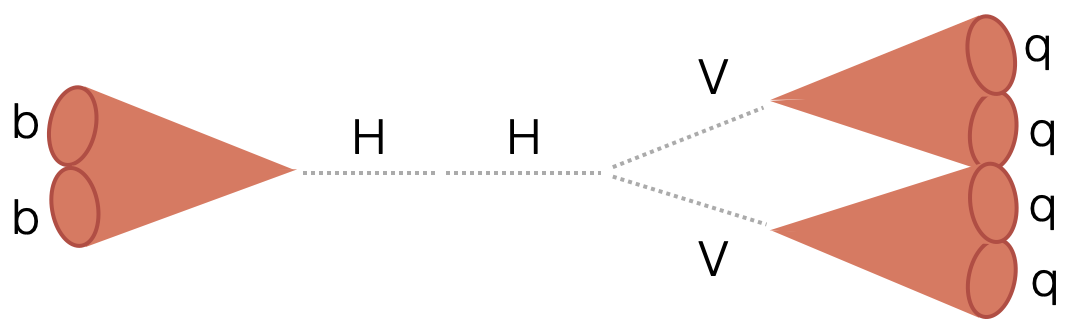
\includegraphics[width=0.48\textwidth]{figures/05-HH/HHbbVV-cartoon.png}
% \hspace{0.19\textwidth}
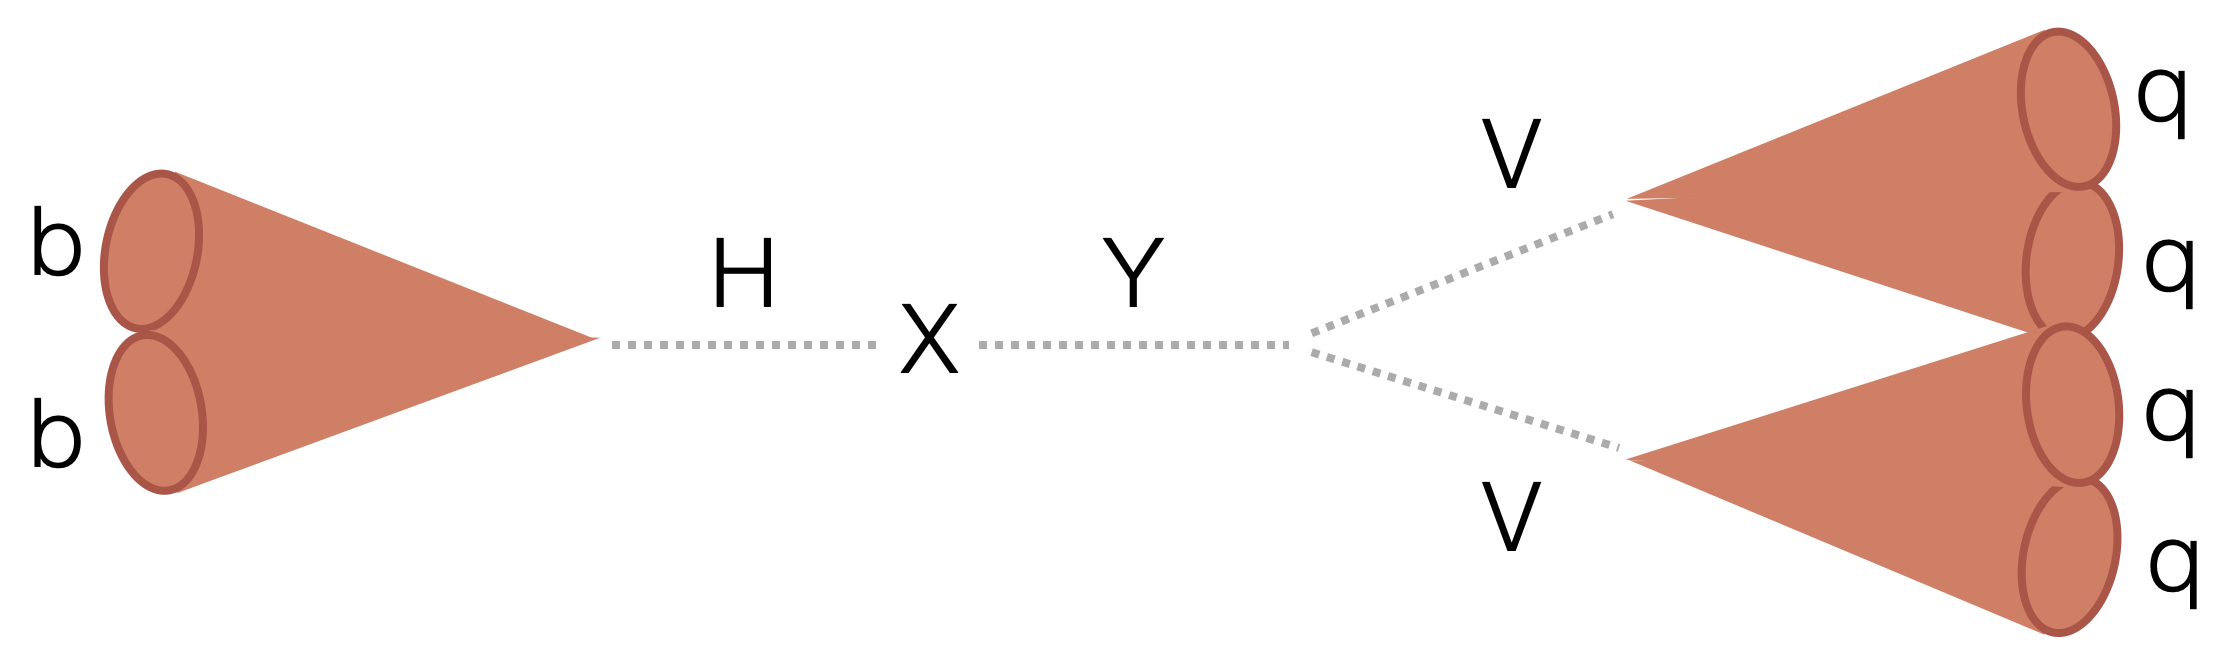
\includegraphics[width=0.48\textwidth]{figures/05-HH/XHYbbVV-cartoon.png}
\caption{The boosted \HHbbVVq (left) and \XHYbbVVq (right) processes.}
\label{fig:05_hhbbvv}
\end{figure}


\section{Introduction}

We now present two searches for the simultaneous production of two highly energetic Higgs bosons using the CMS detector at the LHC and the AI developments described in the previous chapter.
The first search targets \textbf{nonresonant} Higgs pair (\HH) production as predicted by the standard model (SM) to measure critical SM parameters; while the second looks for \textbf{resonant} Higgs (\PH) and Higgs-like (\PY) production resulting from new beyond-SM (BSM) particles (\PX) in the high energy Higgs sector, to explain mysteries such as the hierarchy problem and matter-antimatter asymmetry.

In the SM, \HH production is expected to be an extremely rare process: out of the 1,000,000,000,000,000 collisions observed by CMS in Run 2 of the LHC, only 6000 of them are expected to produce two Higgs bosons.
On top of that, the each Higgs decays into a variety of different particles, or ``final states'', splintering the signal further into myriad different experimental signatures, or ``channels'' (shown in Figure~\ref{fig:05_hhbrs}).

However, as detailed in Chapter~\ref{sec:01_higgs}, its measurement can uniquely probe the Higgs trilinear self- (\cl) and quartic two-vector-boson- (\cvv) couplings, the former being critical to understanding the Higgs potential and the nature of electroweak symmetry breaking.
Indeed, this is why it is considered one of the flagship measurements of the CMS and ATLAS experiments' HL-LHC programs.
Due to the rarity of \HH production, the current measurements of these couplings are some of our least precise, with \cl constrained to $[-1.39, 7.02]$ and \cvv to $[0.62, 1.42]$ times their SM prediction at $95\%$ confidence level (\CL) by CMS~\cite{CMS-PAS-HIG-20-011}.
This calls for new, innovative techniques to cover the vast phase space of \HH decays.

This chapter presents one such idea, measuring for the first time the all-hadronic \HHbbVV channel: where one Higgs decays into a pair of bottom quarks (\bbbar), and the other into a pair of vector bosons (\VV), which then decay into four quarks (\qqqq) (Figure~\ref{fig:05_hhbbvv}, left).
While not a traditional ``golden channel'' (Chapter~\ref{sec:05_smhh_golden_channels}), due to its complicated and noisy experimental signature, by 1) targeting the extremely high energy \HH regime, where both Higgs bosons are produced highly Lorentz-boosted; and 2) exploiting and developing advanced ML techniques for identifying such boosted Higgs bosons (Chapter~\ref{sec:05_jet_tagging}), we are able to achieve competitive sensitivity to boosted \HH production and the \cvv coupling.
% In particular, we showcase the development and application of an attention-based ParticleTransformer model~\cite{Qu:2022mxj} to identify boosted \hvvq jets, which has proven to be a critical component of not only this analysis, but many ongoing boosted Higgs searches in CMS.

By measuring \HH production and couplings, especially in the boosted regime, the nonresonant search is also indirectly sensitive to new physics in the very high energy Higgs sector, which could manifest as deviations from SM predictions.
To complement this, this chapter also presents a \textit{resonant} search for direct evidence of such new physics, in the form of new particles in the Higgs sector: specifically, a heavy scalar \PX which can decay into a Higgs and Higgs-like boson \PY, in the same final state (Figure~\ref{fig:05_hhbbvv}, right).
As described in Chapter~\ref{sec:05_bsmxhy}, such additions to the Higgs sector are motivated by a variety of BSM models, such as composite Higgs models, supersymmetry, and extra dimensions, to solve the matter-antimatter asymmetry and hierarchy problems.
The \bbvv channel is particularly important for this search because for heavy \PY boson masses, assuming SM Higgs-like couplings, the \yvv decay modes are completely dominant (Figure~\ref{fig:01_sm_higgs_hbrs}).
Hence, the \bbvv channel is expected to have the highest branching fraction.
The resonant search exploits the same techniques and developments as the nonresonant, but searches more broadly for excesses, or ``bumps'', in the resonant di-Higgs mass spectrum corresponding to the mass of the new particle \PX.

% Together, these two searches represesnt a sensitive and innovative approach to studying the very high energy Higgs sector at the LHC, and are a testament to the power of combining advanced ML techniques with traditional experimental methods to probe the most fundamental questions in particle physics.
This chapter is organized as follows.
% Section~\ref{sec:05_smhh} and~\ref{sec:05_bsmxhy} discuss SM \HH  and BSM \XHY production, respectively, and the motivations for their all-hadronic \bbvv channels.
Section~\ref{sec:05_analysis_strategy} outlines the analysis strategy for both searches, based on the ML techniques described in Chapter~\ref{sec:05_jet_tagging} for identifying boosted Higgs jets, before detailing the online and offline event selection for both the nonresonant and resonant searches in Section~\ref{sec:05_selection}.
The background estimation strategy and systematic uncertainties are then described in Sections~\ref{sec:05_bgestimation} and~\ref{sec:05_hh_systematics}, respectively, followed by the Run 2 results of the nonresonant and expected results of the resonant searches in Section~\ref{sec:05_results}.
Finally, we conclude in Section~\ref{sec:05_outlook} with a summary and outlook for boosted \HH analyses in Run 3 and the HL-LHC.
%  identification of boosted Higgs jets using ML techniques
% , with Section~\ref{sec:05_hww_tagger} describing specifically the development and calibration of the boosted \hyvv tagger.
% Finally, Sections~\ref{sec:05_results} and~\ref{sec:05_outlook} conclude with the Run 2 results and outlook for boosted \HH analyses in Run 3 and the HL-LHC.

\section{Overview of analysis strategy}
\label{sec:05_analysis_strategy}

Looking for all-hadronic decays is challenging because of the large QCD multijet background.
By searching for boosted \HHY production, where the final state particles for each Higgs boson produce a single merged wide-radius jet, this background is exponentially reduced.
Furthermore, in this regime, deep learning techniques can be extremely effective in identifying these unique merged wide-radius signal jets using low-level reconstructed particle and vertex data; indeed, key components of this search are the development and application of such techniques for identifying boosted Higgs jets.

For both the nonresonant and resonant searches, triggers and a loose offline preselection for boosted jets are first applied, selecting for two high \pt wide-radius jets with at least one loosely \bbbar-tagged.
The key discriminating features between our signals and the predominantly QCD background are the masses of the two jets (plus the dijet mass in the resonant search) and \bbbar and \VV tagging scores.
As described in Chapter~\ref{sec:05_jet_tagging}, we use ParticleNet-based mass regression to improve the mass resolution of the two jets, and the established ParticleNet and new Particle Transformer mass-decorrelated taggers for \bbbar and \VV tagging, respectively.

Following the event selection, which uses a combination of these features, QCD remains the dominant background in the signal regions.
The shape and normalization of this background are predicted from data in control regions, defined by inverting tagger selections, multiplied by transfer factors assumed to be smoothly parametrized functions.
Smaller contributions from top quark and vector boson backgrounds are predicted from MC simulations.

For the nonresonant analysis, an event-level boosted decision tree (BDT) is trained to further discriminate between the HH signals and the QCD multijet and top backgrounds.
As the boosted regime is particularly sensitive to high \kapvv deviations, the BDT optimized simultaneously for both the SM ggF HH signal as well as the BSM VBF signal with \kapvv = 0, and includes information about smaller-radius forward jets which are unique to the VBF mode.
The shape of the \bbbar~jet mass exhibits a resonance peak for the HH signal (with better resolution than the \VV jet mass) and thus it is chosen as the observable used in the final step of the signal extraction procedure.
The control region for the QCD background is defined by inverting the \bbbar tagger cut.

In the resonant case, the two tagger scores, along with a selection around the Higgs mass window on the \bbbar-tagged jet, are used to define the signal region.
The signal is then extracted from the 2D distribution of the dijet mass and \ww-tagged jet mass, with the QCD background predicted from a control region with both tagger scores inverted.
As the analysis is currently blinded in the signal region, secondary validation pass and fail regions are defined with the same selections above, except in the sidebands of the Higgs mass.
These are used to estimate the background in the signal region and derive expected sensitivities and upper limits.


\section{Event Selection}
\label{sec:05_selection}

The primary physics objects considered in this analysis are large-radius, AK8 jets representing the two Higgs bosons.
AK4 jets are also used in the online triggers and to identify nonresonant VBF \HH production.
As we do not expect any isolated leptons in our signal, events containing any isolated electrons and muons are vetoed.
The online trigger selections are described in Section~\ref{sec:05_triggers}, and the offline selections for the nonresonant and resonant searches in Sections~\ref{sec:05_selection_nonresonant} and~\ref{sec:05_selection_resonant}, respectively.

\subsection{Triggers}
\label{sec:05_triggers}

No dedicated online trigger algorithms were available in Run 2 for boosted Higgs classification.
Instead, a combination of high level triggers (HLTs) is considered, which require high hadronic activity and/or AK8 jets with high transverse momentum, as well as jet mass and/or \Pb-tagging requirements.
The efficiencies of these triggers as a function of AK8 jet \pt, soft-drop mass~\cite{Larkoski:2014wba}, and \bbbar-tagging score are measured in data in an unbiased semi-leptonic \ttbar region, defined using single muon triggers and offline selections on the muon and an AK8 jet.
This measurement is shown in Figure~\ref{fig:05_triggers_eff_2018} for the 2018 dataset.
The triggers are generally fully efficient for jet $\pt > 500\GeV$, while for $\pt < 400\GeV$ the efficiency is $\lesssim 10\%$.
\textbf{This is a significant limitation of the analysis} and generally of boosted Higgs searches in Run 2, which is addressed in Run 3 by the introduction of dedicated triggers for boosted Higgs searches~\cite{Varghese:2023bue}.

\begin{figure}[hbt!]
\centering
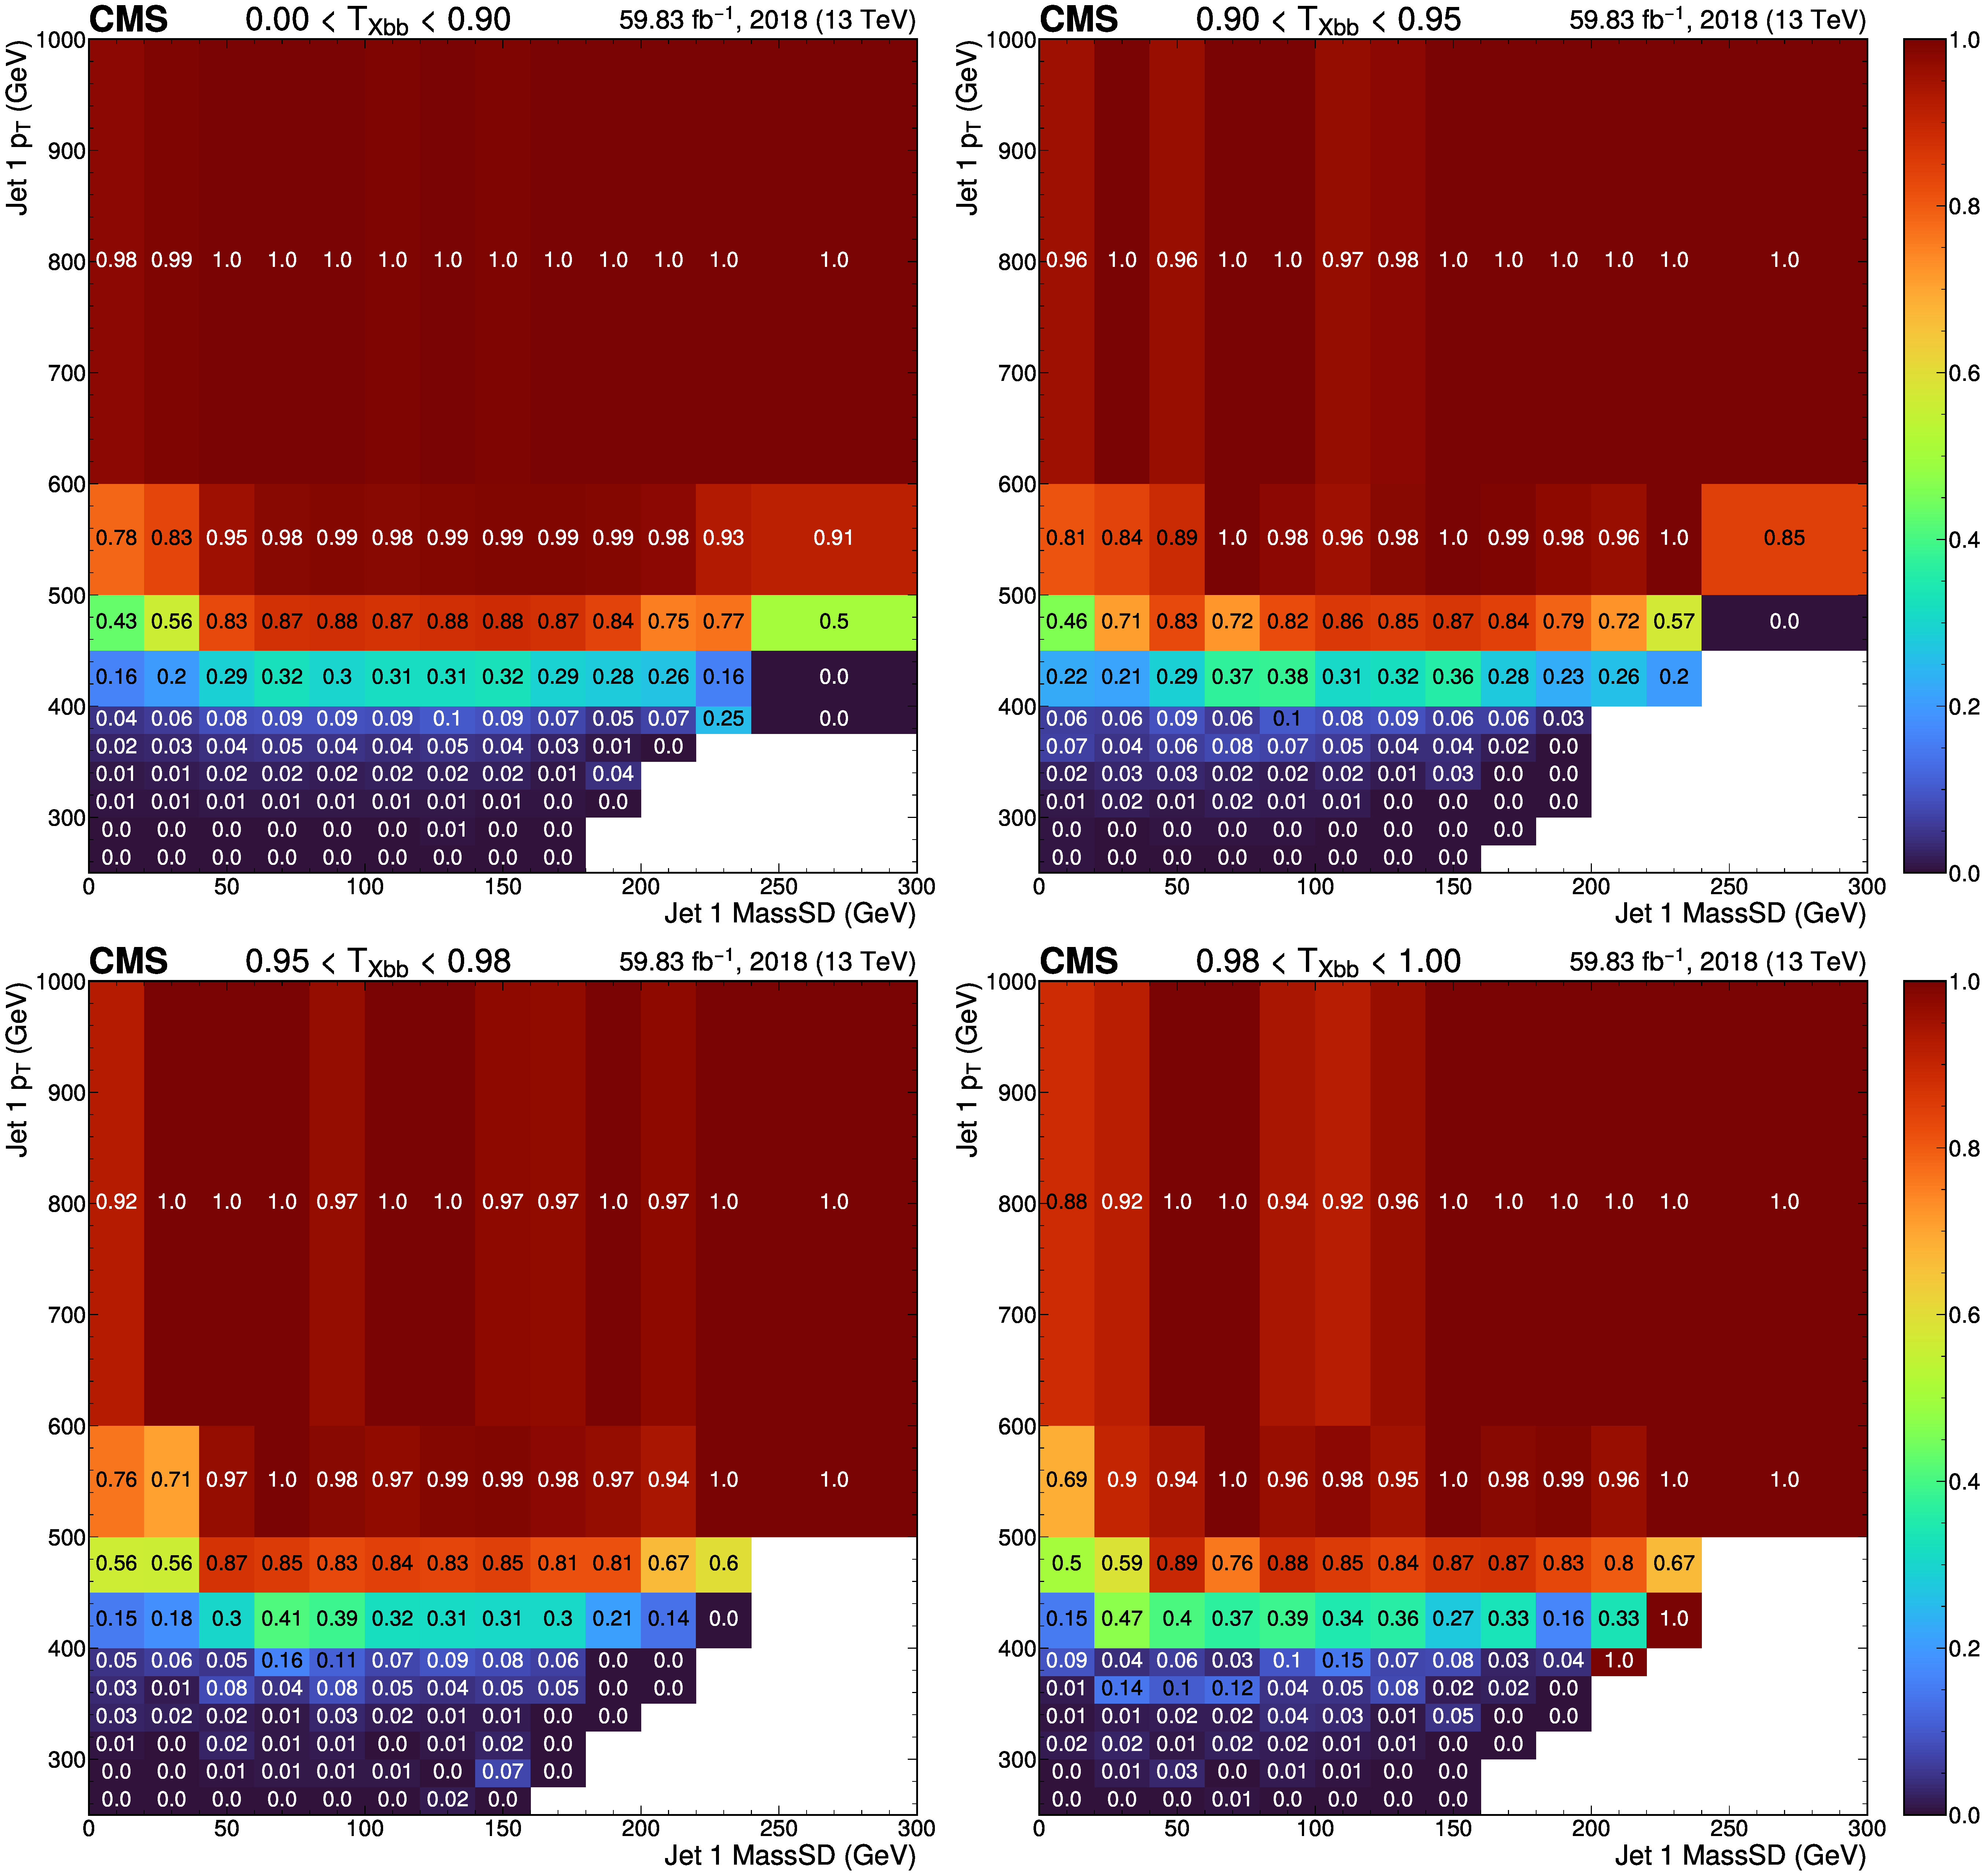
\includegraphics[width=\textwidth]{figures/05-HH/selection/2018_txbb_effs.pdf}
\caption{Trigger efficiencies for the 2018 dataset measured in bins of the AK8 jet \pt, soft drop mass (MassSD) and \TXbb score.
\label{fig:05_triggers_eff_2018}
}
\end{figure}

\subsection{Nonresonant offline selection}
\label{sec:05_selection_nonresonant}

In the nonresonant analysis, both the \hbb and \hvv decays are targeted through an offline selection for two highly boosted AK8 jets with a minimum \pt of $300\GeV$ and $\abs{\eta} < 2.4$.
ParticleNet is used to isolate the signal \hbb jets against background QCD jets, using the \TXbb discriminant derived from its outputs (Eq.~\ref{eq:05_txbb}), while our new GloParT model is leveraged to identify the \hvvq jet.
% , we introduce a new attention-based neural network called ``GloParT'', based on the ParticleTransformer (ParT) architecture~\cite{Qu:2022mxj}, described below in Section~\ref{sec:05_boosted_jets}.
Both networks have been decorrelated from the mass of the jets by enforcing a uniform distribution in jet mass and \pt in the training samples~\cite{CMS:2023tlv}, to aid with their calibration.
Additionally, as the jet mass resolution is crucial to the sensitivity of the search, we optimize the mass reconstruction for all AK8 jets using the ParticleNet-based regression algorithm, the output of which we refer to as \mreg.
The jet with the higher (lower) \TXbb score is considered the \bbbar- (\VV-) candidate jet.

The VBF process produces two, likely forward, jets with large invariant masses and pseudorapidity separations.
To identify this mode, we select up to two AK4 jets per event, required to have $\pt > 25\GeV$, $\abs{\eta} < 4.7$, and a $\Delta R$ separation of 1.2 and 0.8, respectively, from the \bbbar- and \VV-candidate AK8 jets.
The pseudorapidity separation between and invariant mass of the two highest \pt jets passing these requirements are used as input variables in a boosted decision tree (BDT) to discriminate against QCD and other backgrounds.
Other input variables include outputs from the GloParT tagger and the two selected AK8 jet kinematics.
The variables are optimized to provide the highest BDT performance while remaining decorrelated from the \bbbar-candidate jet's mass.

The BDT is optimized simultaneously for both the SM ggF and BSM VBF $\kapvv=0$ signals, and separate ``ggF'' and ``VBF'' signal regions are defined using the BDT probabilities for the respective processes, referred to as \ggfbdt and \vbfbdt.
Concretely, the VBF region is defined by selections on the \TXbb and \vbfbdt discriminants, corresponding to VBF signal (background) efficiencies of 40\% ($\approx 0.1\%$) and 20\% ($\approx 0.003\%$), respectively, chosen to optimize the expected exclusion limit on the VBF signal.
The ggF region is defined by a veto on events passing the VBF selections plus selections on the \TXbb and \ggfbdt discriminants, corresponding to ggF signal (background) efficiencies of 60\% ($\approx 0.3\%$) and 7\% ($\approx 0.01\%$), respectively, similarly chosen to optimize the limit on the ggF signal.
These selections are henceforth referred to as the ggF and VBF \TXbb and BDT working points (WPs).
The \TXbb discriminant's signal efficiencies are calibrated using boosted gluon splitting to bottom quark ($\Pg\to\bbbar$) jets in data and simulations~\cite{CMS:2023tlv}, with \pt-dependent scale factors and uncertainties applied to the \HH signals.
The uncertainty on the BDT signal efficiency is dominated by that of the GloParT tagger and is calibrated based on a new technique using the ratio of the primary Lund jet plane~\cite{Dreyer:2018nbf} densities of each individual quark-subjet, described below in Section~\ref{sec:05_hww_calibration}.

The search is performed by constructing a likelihood in the pass region as a function of the \hbb-candidate jet's regressed mass (\mregbb).
The QCD multijet background contribution in the pass region is estimated through data in a ``fail'' region, defined using the same baseline selections on the two AK8 jets, but with the \TXbb selection inverted, as described in Section~\ref{sec:05_bgestimation} below.
A summary of all offline selections is provided in Table~\ref{table:05_selections_nonresonant}, and the signal and fail region selections in terms of the \TXbbbb and BDT scores are illustrated in Figure~\ref{fig:05_selection_nonresonant}.


\begin{table}[htbp!]
    \unless\ifdefined\HCode
        \renewcommand{\arraystretch}{1.4}
    \fi
    \centering
    \caption{Offline selection criteria for the signal and fail nonresonant analysis regions.}
    \begin{tabular}{c|c|c}
    \toprule
    VBF Region &  ggF Region &  Fail Region \\ \midrule
    \multicolumn{3}{c}{\begin{tabular}[c]{@{}c@{}}
        No electrons or muons \\[3mm]

        $\geq 2$ AK8 jets \\
        $\pt > 300$\GeV (all jets) \\
        $|\eta| < 2.4$ (all jets) \\
        $50 < \mreg < 250\GeV$ (all jets) \\
        $\TXbb > 0.8$ (at least one jet) \\[3mm]

        Jet assignment: \\
        \hbb: highest $\TXbb$ score \\
        \hvv: out of remaining jets, highest GloParT score
    \end{tabular}} \\\midrule
    % Selection criteria rows
    & Not passing VBF selections & \\
    $\TXbbbb \geq$ VBF \TXbb WP & $\TXbbbb \geq$ ggF \TXbb WP & $\TXbbbb <$ ggF \TXbb WP \\
    $\vbfbdt \geq$ VBF BDT WP & $\ggfbdt \geq$ ggF BDT WP & \\ \cbottomrule
    \end{tabular}
    \label{table:05_selections_nonresonant}
\end{table}

\begin{figure}[htb!]
    \centering
    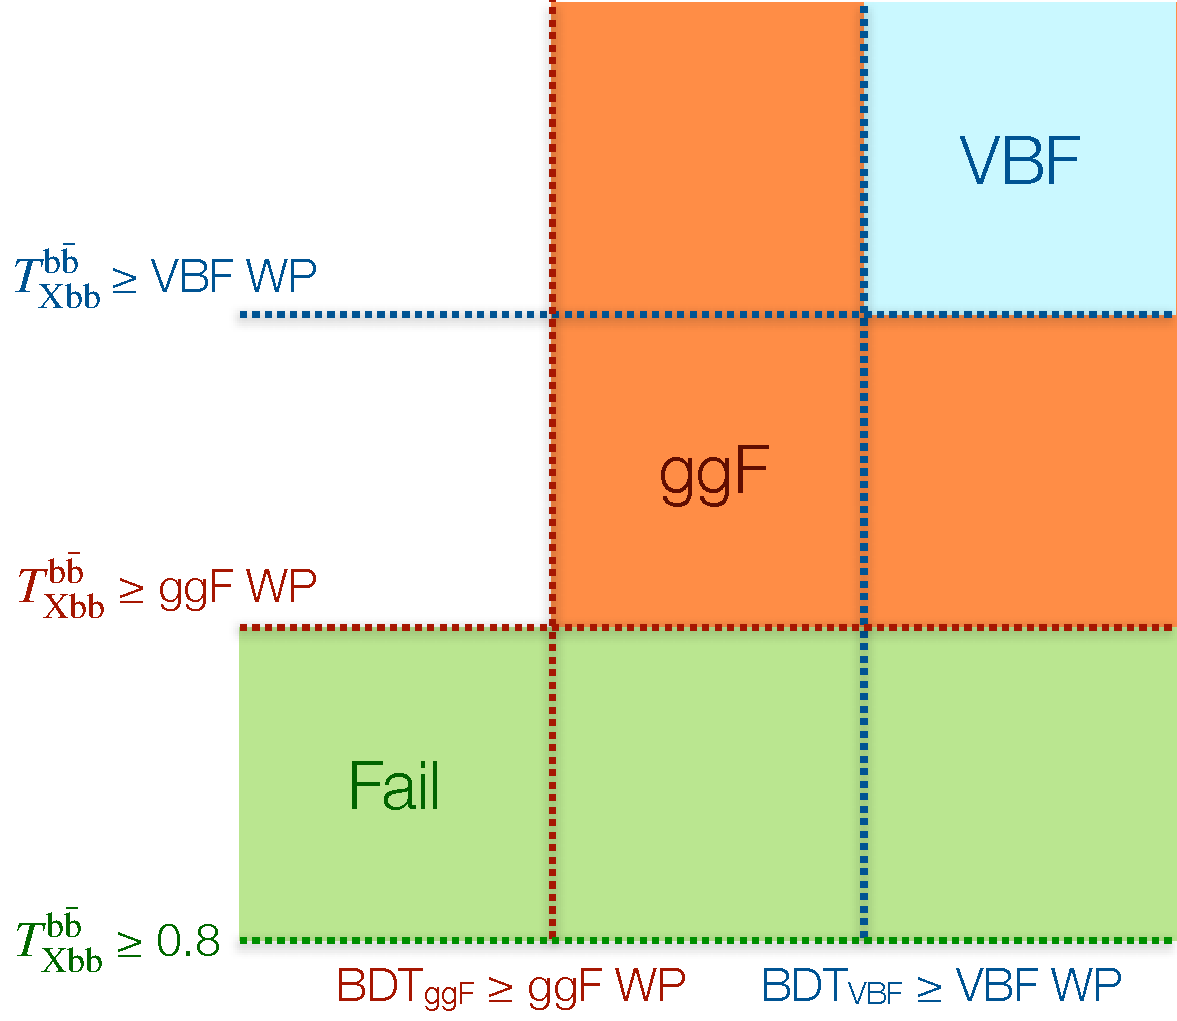
\includegraphics[width=0.7\textwidth]{figures/05-HH/selection/Nonresonant_Selections.pdf}
    \caption{Illustration of the signal and fail nonresonant analysis region selections in terms of the \TXbbbb and BDT scores.}
    \label{fig:05_selection_nonresonant}
\end{figure}


\subsection{Resonant offline selection}
\label{sec:05_selection_resonant}

The resonant analysis similarly selects for two wide-radius jets representing the two \hbb and \yvv processes.
Specifically, we select for two boosted AK8 jets with $\pt \geq 350\GeV$, with at least one of $\pt \geq 400 \GeV$, and pseudorapidity $|\eta| \leq 2.4$.
Out of all AK8 jets in the event passing these requirements, the one with the highest \TXbb discriminant score is considered our \hbb candidate jet, and is required to pass the high purity WP and have a jet mass close to the SM Higgs mass: $110 \leq \mathrm{mass} < 145\GeV$.
As in the nonresonant case, the jet mass resolution is crucial to the sensitivity of the search and hence we use the ParticleNet-based regression algorithm to reconstruct the jet mass, \mreg, here as well.

The mass-decorrelated GloParT tagger is again used to identify the \yvvq jet, using the discriminant \THWW targeting the \VVq final state derived from its outputs (Eq.~\ref{eq:05_thww}).
The AK8 jet passing the above \pt and $\eta$ kinematic selections with the highest \THWW score is considered the \yvv candidate jet,\footnote{\label{bbvvconflictnote}In the rare ($<0.1\%$ of signal events) case where the same jet has the highest \TXbb and \THWW score, that jet is considered the \hbb candidate, and the second-highest \THWW scoring jet is the \yvv candidate.}
and is required to have a \THWW score $> 0.6$, corresponding to a $\approx 60\%$ ($\approx 1\%$) signal (background) efficiency.
The signal efficiency is calibrated based the Lund jet plane as described in Chapter~\ref{sec:05_hww_calibration}.
All the \pt and tagger selections were jointly optimized for the lowest expected exclusion limits for a range of \mxmy points.

The search is performed in events passing these selections, referred to as the signal or ``pass'' region, in the 2D plane of the \VV-candidate jet regressed mass (\mregvv) and the invariant mass of the \bbbar- and \VV-candidate jets (\mjj), representing the potential \PY and \PX boson masses, respectively.
An orthogonal control, or ``fail'', region is defined by inverting the two tagger selections for both jets to estimate the QCD background in the pass region, as detailed in Section~\ref{sec:05_bgestimation}.
Finally, separate ``validation'' pass and fail regions using the \hbb candidate jet's mass sidebands are used to validate the background estimation technique before unblinding the analysis.
A summary of the offline selections is provided in Table~\ref{table:EvtSel-mergedY}.


\begin{table}[htbp!]
    \unless\ifdefined\HCode
        \renewcommand{\arraystretch}{1.4}
    \fi
    \caption{Offline selection criteria for analysis regions for the fully-merged \PY topology.}
    \label{table:EvtSel-mergedY}
    \centering\resizebox{\textwidth}{!}{
    \begin{tabular}{c|c|c|c}
    \toprule
    \multicolumn{2}{c|}{Signal Region} & \multicolumn{2}{c}{Validation Region} \\ \midrule

    \multicolumn{4}{c}{\begin{tabular}[c]{@{}c@{}}
    $\geq 2$ AK8 jets \\
    $\pt > 350$\GeV (all jets) \\
    $|\eta| < 2.4$ (all jets) \\
    $\pt > 400$\GeV (jet leading in \pt) \\[3mm]

    Jet assignment: \\
    \hbb: highest $\TXbb$ score \\
    \yvv: out of remaining jets, highest $\THWW$ score
    \end{tabular}} \\
    \midrule
    \multicolumn{2}{c|}{$110 \leq \mregbb < 145\GeV$} & \multicolumn{2}{c}{$92.5 \leq \mregbb < 110\GeV$ or $145 \leq \mregbb < 162.5\GeV$} \\
    \midrule
    Pass & Fail & Pass & Fail \\ \midrule
    $\TXbb \geq \mathrm{HP\ WP}$ & $\TXbb < \mathrm{HP\ WP}$ & $\TXbb \geq \mathrm{HP\ WP}$ & $\TXbb < \mathrm{HP\ WP}$ \\
    $\THWW \geq 0.6$ & $\THWW < 0.6$ & $\THWW \geq 0.6$ & $\THWW < 0.6$ \\
    \cbottomrule
    \end{tabular}
    }
\end{table}

\section{Background estimation}
\label{sec:05_bgestimation}

The QCD multijet background is the primary background of both searches.
It is estimated with a data-driven approach, using the shape of the data minus other MC backgrounds, whose uncertainties are incorporated into the fit, in a control region multiplied by a polynomial transfer factor to the signal regions, whose order is determined by an $F$-test.
This is described in more detail below.
The parameters of the transfer factor are estimated with a simultaneous fit in the signal and fail regions.
Other minor backgrounds include top quark and vector boson plus jets, which are estimated from MC simulation.

Correction factors are applied to the W and Z boson samples to match the generator-level \pt distributions with those predicted by the highest available order in the perturbative expansion.
The $\PW+$jets and $\PZ+$jets MC samples are corrected to approximately NNLO in QCD and then further reweighted to incorporate the reduction of the cross section at high \pt due to higher-order electroweak effects (EWK).

The QCD event yields in the signal, or ``pass'', and fail regions are related by a smoothly parametrized transfer factor $\rpf$:
\begin{equation}
n(\mathrm{QCD})^{\mathrm{pass}}_b = \rpf(m)\, n(\mathrm{QCD})^{\mathrm{fail}}_b,
\end{equation}

where $n(\mathrm{QCD})_b$ is the QCD yield in bin $b$, and $n(\mathrm{QCD})^{\mathrm{fail}}_b$ is estimated to be the data in the fail region minus non-QCD backgrounds.
In the nonresonant case, separate transfer factors are used for each signal region $R$ ($\in$ \{ggF, VBF\}), each of which is parametrized by the coefficients $a^R_k$ of the set of $n^R + 1$ Bernstein basis polynomials $b_{k, n^R}$ of order $n^R$ in \mregbb:
\begin{equation}
R^{\mathrm{Region\ R}}_{P/F\ \textrm{nonresonant}}(\mregbb) = \sum^{n^R_\mregbb}_{k=0} a^R_k b_{k, n^R_\mregbb}(\mregbb),
\end{equation}
while in the resonant case it is generalised to two dimensions, as a function of \mjj and \mregvv:
\begin{equation}
R_{P/F\ \textrm{resonant}}(\mjj, \mregvv) = \sum^{n_\mjj}_{k=0} \sum^{n_\mregvv}_{l=0} a_{k,l} \big[ b_{k, n_\mjj}(\mjj)\, b_{l, n_\mregvv}(\mregvv)\big].
\end{equation}

The optimal orders of the polynomials are determined to be $n^{\mathrm{ggF}}_\mregbb = 0$, $n^{\mathrm{VBF}}_\mregbb = 1$, $n_\mjj = 2$, and $n_\mregvv = 1$ by a Fisher F-test.
This iteratively tests each polynomial order, starting from the lowest considered, against higher order polynomials to see if the latter provide significantly better fits.
The lowest order tested is 0 for all but the nonresonant VBF region, for which we require the transfer factor to be at least linear to account for observed shift in the simulated QCD \mregbb shape (due to the higher \mHH phase space of this region).

\section{Systematic uncertainties}
\label{sec:05_hh_systematics}

We consider several sources of theoretical and experimental systematic uncertainties on the signal and background modelling in the signal regions, which are summarized in Table~\ref{tab:05_hh_systematics}.
Overall, the dominant source of uncertainty on the \HH signal strength is the statistical uncertainty in the QCD multijet background estimation, driven by the limited signal region sample size.
This uncertainty has an impact on the best-fit signal strength of 50\% (38\%) relative to the overall uncertainty in the nonresonant (resonant) analyses.

The uncertainties on the signal efficiency of \hbb and \hvv are also significant.
The \hbb efficiency scale factors and uncertainties are measured for data versus simulation in a control region dominated by $\Pg\to\bbbar$ jets~\cite{CMS:2023tlv} and represent a 10\% (15\%) relative impact.
The \hyvv efficiency scale factor and uncertainty measurements are described in Chapter~\ref{sec:05_hww_calibration} and vary depending on the production mode and different coupling strengths of the nonresonant \HH signal, and the \PX and \PY masses of the \XHY signal.
Measured scale factors and uncertainties are shown in Table~\ref{tab:05_hh_nonres_part_ljp_sfs} and Table~\ref{tab:05_hh_res_part_ljp_sfs}, respectively.
Overall, the \hyvv signal efficiencies represent around a 23\% (50\%) relative impact in the nonresonant (resonant) analyses.

Other significant sources of experimental uncertainty include the scale and resolution of the regressed jet mass and reconstructed jet energy~\cite{CMS-DP-2021-033} in data versus simulations.
Jet mass corrections and uncertainties are measured in a control region enriched in \ttbar events, using AK8 jets originating from hadronic \PW boson decays~\cite{CMS-PAS-B2G-21-001}, and with a 7\% (15\%) impact, while jet energy corrections and uncertainties constitute 2\%.
Finally, there are large statistical uncertainties related to the MC simulations of the subdominant top quark and vector boson backgrounds, reaching $30\%$ in some bins of the signal regions; these have roughly a 10\% impact.

On the theoretical side, there is a large uncertainty related to the nonresonant \HH production cross sections, which has a relative impact of up to 24\% on best-fit signal strength.
Uncertainties related to the parton showering performed using \PYTHIA 8~\cite{Mrenna:2016sih} are propagated to the MC kinematic distributions and have a 15\% (5\%) impact, while QCD renormalization and factorization scale uncertainties are estimated by considering the envelope of distributions obtained by varying the scales by a factor of $2$ and constitute a 5\% impact.

Subdominant sources considered include uncertainties related to parton distribution functions (PDFs), \PH branching fractions, luminosity~\cite{CMS-LUM-17-003,CMS-PAS-LUM-17-004,CMS-PAS-LUM-18-002}, pileup interactions, and trigger efficiencies, which have sub-percent-level impacts.

\begin{table}[htb!]
    \caption{Summary of the effect of different systematic uncertainties on the signal or background yields.}
    \label{tab:05_hh_systematics}
    \centering
    \resizebox*{\textwidth}{!}{
        \begin{tabular}{ccc}
            \toprule
            Source                                      & Processes affected & Uncertainty (combined \%) \\ \midrule
            ggF \HH production cross section            & ggF \HH            & $+5\%$/$-19\%$            \\
            VBF \HH production cross section            & VBF \HH            & $2.1\%$                   \\
            \hbb branching fraction                     & \HH and \XHY       & $1.25\%$                  \\
            \hvv branching fraction                     & \HH                & $1.53\%$                  \\
            \hbb tagging signal efficiency              & \HH and \XHY       & $7$--$10\%$               \\
            \hvv tagging signal efficiency              & \HH and \XHY       & $16$--$50\%$              \\
            QCD multijet background uncertainty         & QCD multijet       & $10\%$                    \\
            Parton showering                            & All MC             & $1$--$9\%$                \\
            Jet energy scale and resolution             & All MC             & $1$--$3\%$                \\
            Jet mass scale and resolution               & All MC             & $1$--$4\%$                \\
            MC statistical uncertainty                  & All MC             & $1$--$30\%$               \\
            QCD renormalization and factorization scale & All MC             & $7$--$10\%$               \\
            PDF                                         & All MC             & $1$--$4\%$                \\
            Luminosity                                  & All MC             & $1\%$                     \\
            Pileup                                      & All MC             & $1\%$                     \\
            Trigger efficiency                          & All MC             & ${<}1\%$                  \\\cbottomrule
        \end{tabular}
    }
\end{table}


\begin{table}[!ht]
    \begin{center}
        \caption[Signal efficiency scale factors (SFs) and uncertainties for the BDT selection using the Lund jet plane for different nonresonant \HH signals and analysis regions.]{Signal efficiency scale factors (SFs) and uncertainties for the BDT selection using the Lund jet plane for different nonresonant \HH signals and analysis regions.
        Both the total combined uncertainty and the components mentioned in the text are shown.
        }
        \label{tab:05_hh_nonres_part_ljp_sfs}
        \resizebox*{1\textwidth}{!}{
            \begin{tabular}{c|c|c|c|c|c|c}
                \toprule
                \multirow{2}{*}{Signal Region} & \multirow{2}{*}{Process} & \multirow{2}{*}{SF $\pm$ unc.} & \multicolumn{4}{c}{Uncertainty components (fractional)}                                                                 \\ \cline{4-7}
                                               &                          &                                & Ratio MC modeling                          & Ratio statistical & Ratio \pt extrapolation & Subjet matching \\
                \midrule
                \multirow{4}{*}{ggF} & SM ggF \HH & $1.05 \pm 0.24$ & 0.16 & 0.05 & 0.00 & 0.16 \\
& SM VBF \HH & $1.17 \pm 0.45$ & 0.35 & 0.05 & 0.00 & 0.16 \\
& VBF \HH ($\kapvv = 0$) & $1.09 \pm 0.18$ & 0.02 & 0.04 & 0.01 & 0.15 \\
& VBF \HH ($\kapvv = 2$) & $1.10 \pm 0.18$ & 0.02 & 0.05 & 0.01 & 0.15 \\
\hline
\multirow{4}{*}{VBF} & SM ggF \HH & $0.95 \pm 0.28$ & 0.26 & 0.08 & 0.01 & 0.12 \\
& SM VBF \HH & $1.08 \pm 0.46$ & 0.38 & 0.05 & 0.01 & 0.19 \\
& VBF \HH ($\kapvv = 0$) & $0.93 \pm 0.27$ & 0.16 & 0.06 & 0.02 & 0.23 \\
& VBF \HH ($\kapvv = 2$) & $0.94 \pm 0.27$ & 0.16 & 0.05 & 0.02 & 0.23

                \\ \cbottomrule
            \end{tabular}
        }
    \end{center}
\end{table}

\begin{table}[!ht]
    \begin{center}
    \caption[Signal efficiency scale factors (SFs) and uncertainties using the Lund jet plane for a subset of BSM resonant signals, for our \THWW discriminant working point.]{Signal efficiency scale factors (SFs) and uncertainties using the Lund jet plane for a subset of BSM resonant signals, for our \THWW discriminant working point.
    Both the total combined uncertainty and the components mentioned in the text are shown.
    }
    \label{tab:05_hh_res_part_ljp_sfs}
    \resizebox*{1\textwidth}{!}{
        \begin{tabular}{c|c|c|c|c|c}
        \toprule
        \multirow{2}{*}{Process} & \multirow{2}{*}{SF $\pm$ Unc.} & \multicolumn{4}{c}{Uncertainty components (fractional)} \\ \cline{3-6}
         & & Ratio MC modeling                          & Ratio statistical & Ratio \pt extrapolation & Subjet matching \\
        \midrule
        $\PX[1000]\to\PH\PY[125]$ & 0.74 $\pm$ 0.12 & 0.11            & 0.07            & 0.00                  & 0.09                 \\
$\PX[1400]\to\PH\PY[125]$ & 0.74 $\pm$ 0.08 & 0.00            & 0.03            & 0.03                  & 0.10                 \\
$\PX[1400]\to\PH\PY[150]$ & 0.76 $\pm$ 0.08 & 0.04            & 0.04            & 0.02                  & 0.08                 \\
$\PX[1800]\to\PH\PY[125]$ & 0.73 $\pm$ 0.11 & 0.05            & 0.03            & 0.09                  & 0.10                 \\
$\PX[1800]\to\PH\PY[150]$ & 0.74 $\pm$ 0.11 & 0.09            & 0.04            & 0.08                  & 0.08                 \\
$\PX[1800]\to\PH\PY[190]$ & 0.73 $\pm$ 0.12 & 0.12            & 0.03            & 0.09                  & 0.08                 \\
$\PX[2200]\to\PH\PY[125]$ & 0.79 $\pm$ 0.17 & 0.07            & 0.03            & 0.17                  & 0.11                 \\
$\PX[2200]\to\PH\PY[150]$ & 0.73 $\pm$ 0.18 & 0.16            & 0.03            & 0.16                  & 0.09                 \\
$\PX[2200]\to\PH\PY[190]$ & 0.71 $\pm$ 0.21 & 0.23            & 0.05            & 0.17                  & 0.07                 \\
$\PX[2200]\to\PH\PY[250]$ & 0.73 $\pm$ 0.19 & 0.21            & 0.03            & 0.16                  & 0.05                 \\
$\PX[3000]\to\PH\PY[125]$ & 0.75 $\pm$ 0.28 & 0.17            & 0.03            & 0.30                  & 0.14                 \\
$\PX[3000]\to\PH\PY[150]$ & 0.77 $\pm$ 0.26 & 0.10            & 0.04            & 0.31                  & 0.09                 \\
$\PX[3000]\to\PH\PY[190]$ & 0.73 $\pm$ 0.31 & 0.29            & 0.03            & 0.31                  & 0.07                 \\
$\PX[3000]\to\PH\PY[250]$ & 0.71 $\pm$ 0.35 & 0.38            & 0.04            & 0.31                  & 0.04
        \\ \cbottomrule
        \end{tabular}
    }
    \end{center}
\end{table}


% The dominant source of uncertainty on the \HH signal strengths in the nonresonant analysis is the statistical uncertainty on the QCD multijet background estimation, which accounts for 50\% of the overall uncertainty.
% Other sources include the theory uncertainty in the \HH cross section (24\%), the uncertainties in the BDT and \TXbb signal efficiency scale factors (23\% and 15\%, respectively), systematic uncertainties in the parton showering (15\%), and statistical uncertainties in the top quark simulation (8\%).

% The dominant source of uncertainty in the resonant analysis is that of the signal efficiency of the ParticleTransformer \yvvq classifier, accounting for 50\% of the overall uncertainty on the signal strength.
% This is followed by the systematic uncertainty on the QCD background estimate, contributing to 38\% of the overall uncertainty, while other significant sources include uncertainties on the signal efficiency of the ParticleNet \hbb classifier (15\%), the jet mass and energies (15\%), pileup (5\%), and the luminosity (3\%).


\section{Results}
\label{sec:05_results}

\subsection{Nonresonant \texorpdfstring{\HH}{HH} search}
\label{sec:05_results_hh}

A binned maximum likelihood-fit is performed simultaneously in the ggF, VBF, and fail regions, and the post-fit distributions are shown in Figure~\ref{fig:05_results_hh_postfit}, with QCD in the signal regions predicted using the data-driven estimate described in Section~\ref{sec:05_bgestimation}.
Upper limits on the \HH production cross section and constraints on the \kapvv coupling at a 95\% \CL are derived based on the asymptotic formulae for the profile likelihood ratio test statistic and the \CLs criterion, as described in Chapter~\ref{sec:03_stats} and are shown in Figures~\ref{fig:05_results_hh_UL} and~\ref{fig:05_results_hh_UL_k2v}, respectively.
The upper limits on the SM \HH production cross section and for $\kapvv=0$ are observed (expected) to be \hhobs (\hhexp) and \cvvobs (\cvvexp) relative to the theoretical predictions, respectively.
The coupling modifier \kapvv is observed (expected) to be constrained within \kvvobslims (\kvvexplims) at 95\% CL, which represents the second-strongest constraint by CMS to date, behind only the boosted \bbbb analysis.

\begin{figure}[hbt!]
\centering
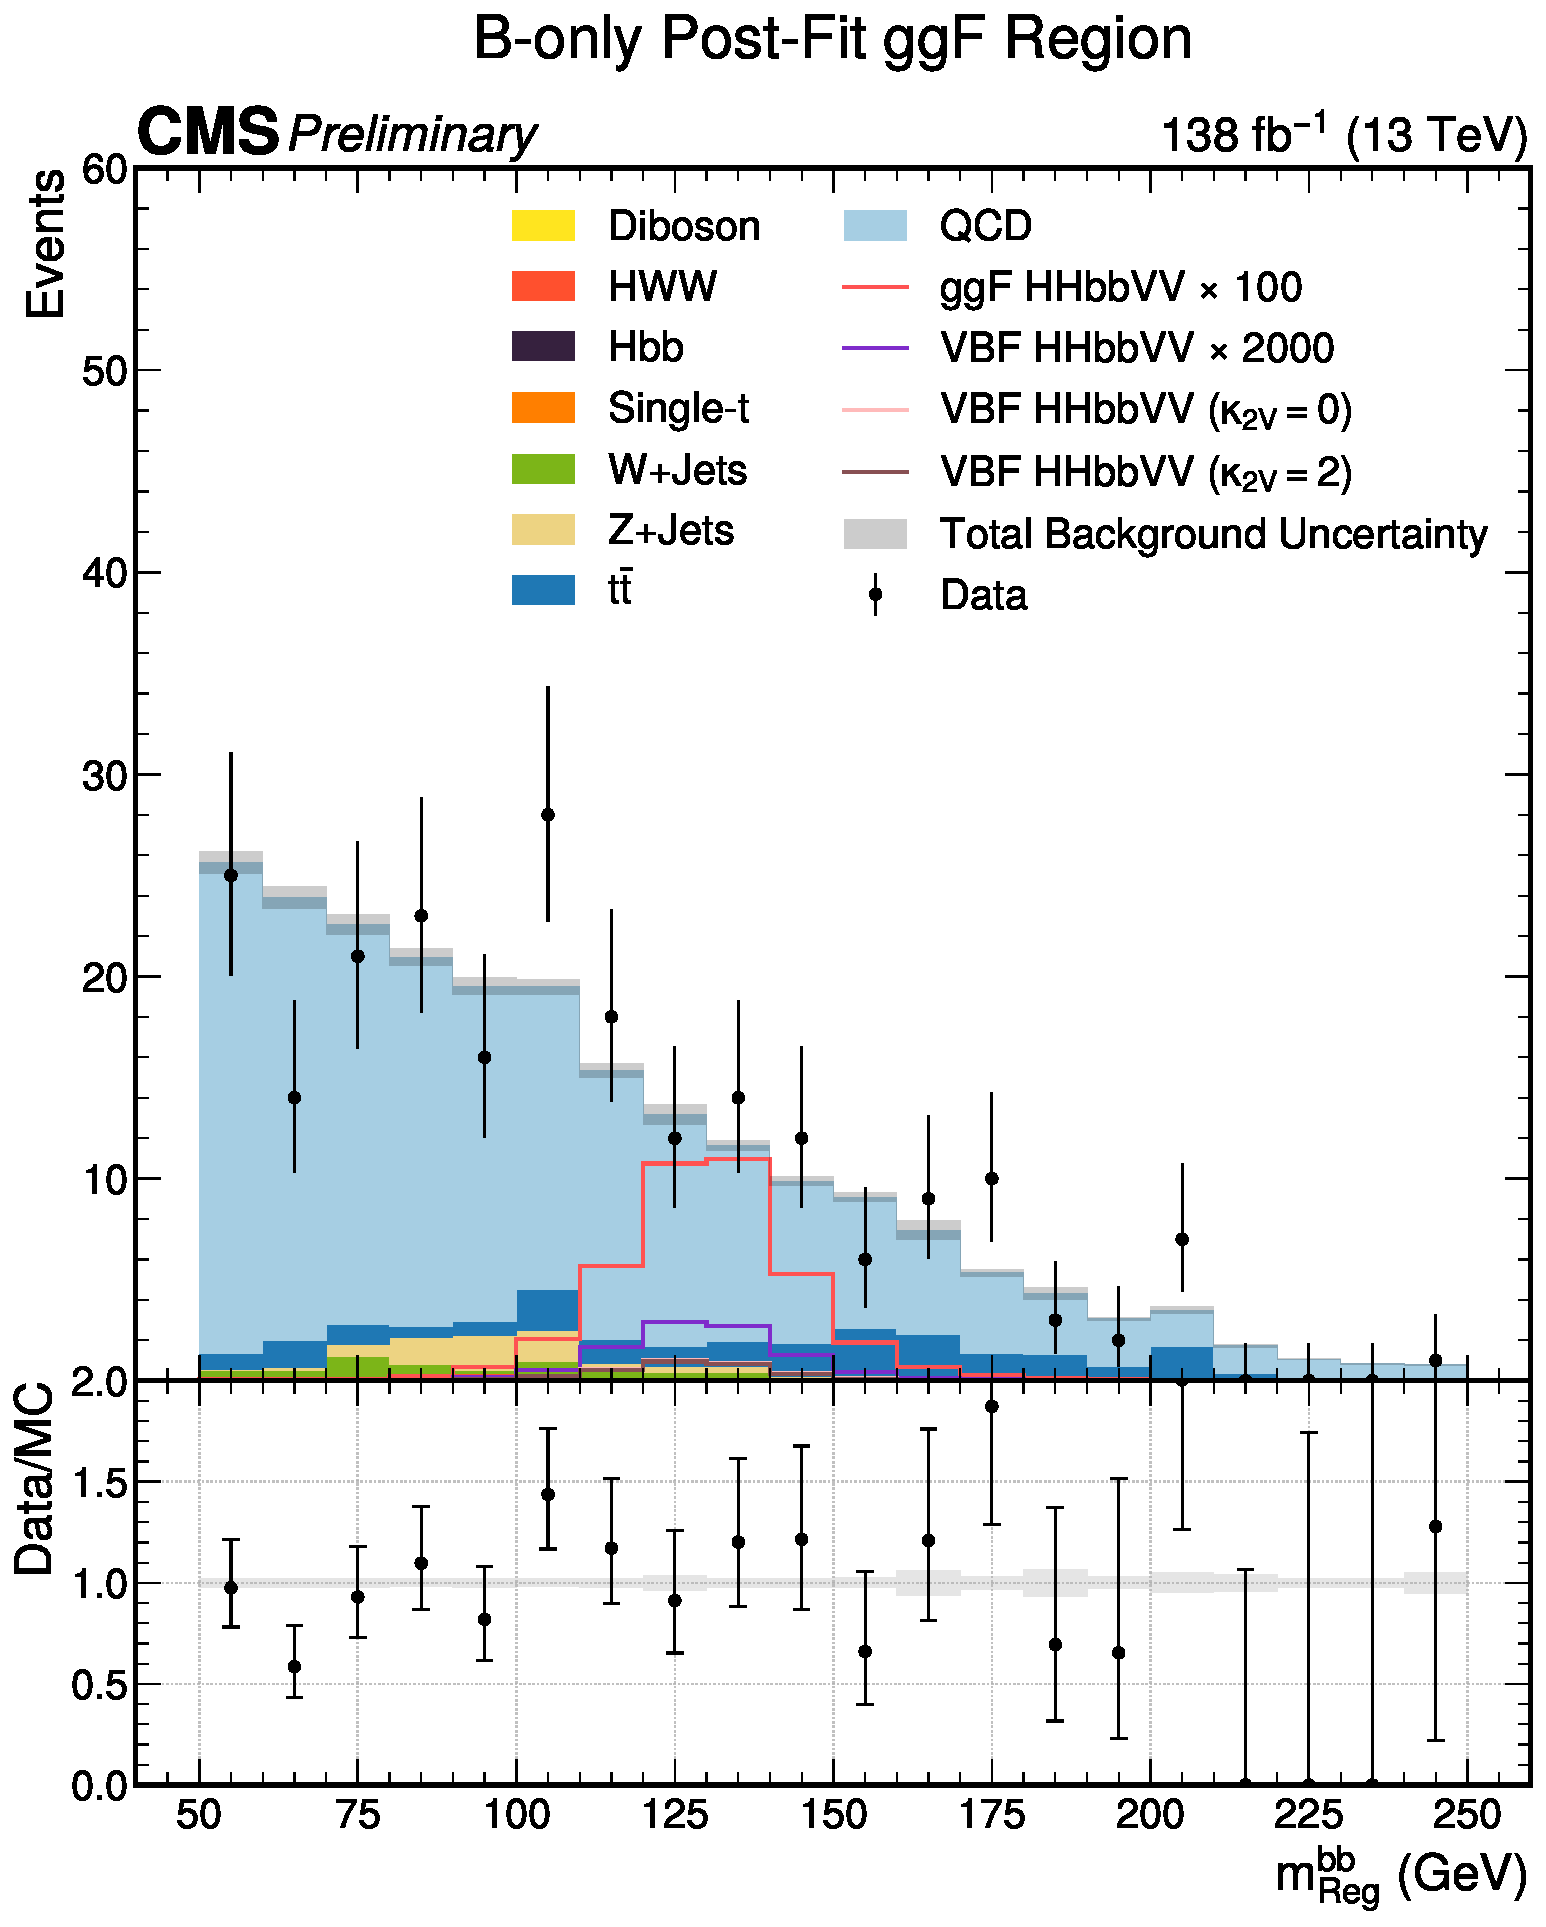
\includegraphics[trim={0 0 0 15mm},clip,width=0.49\textwidth]{figures/05-HH/results_nonres/postfit_passggf_bbFatJetParticleNetMass.pdf}
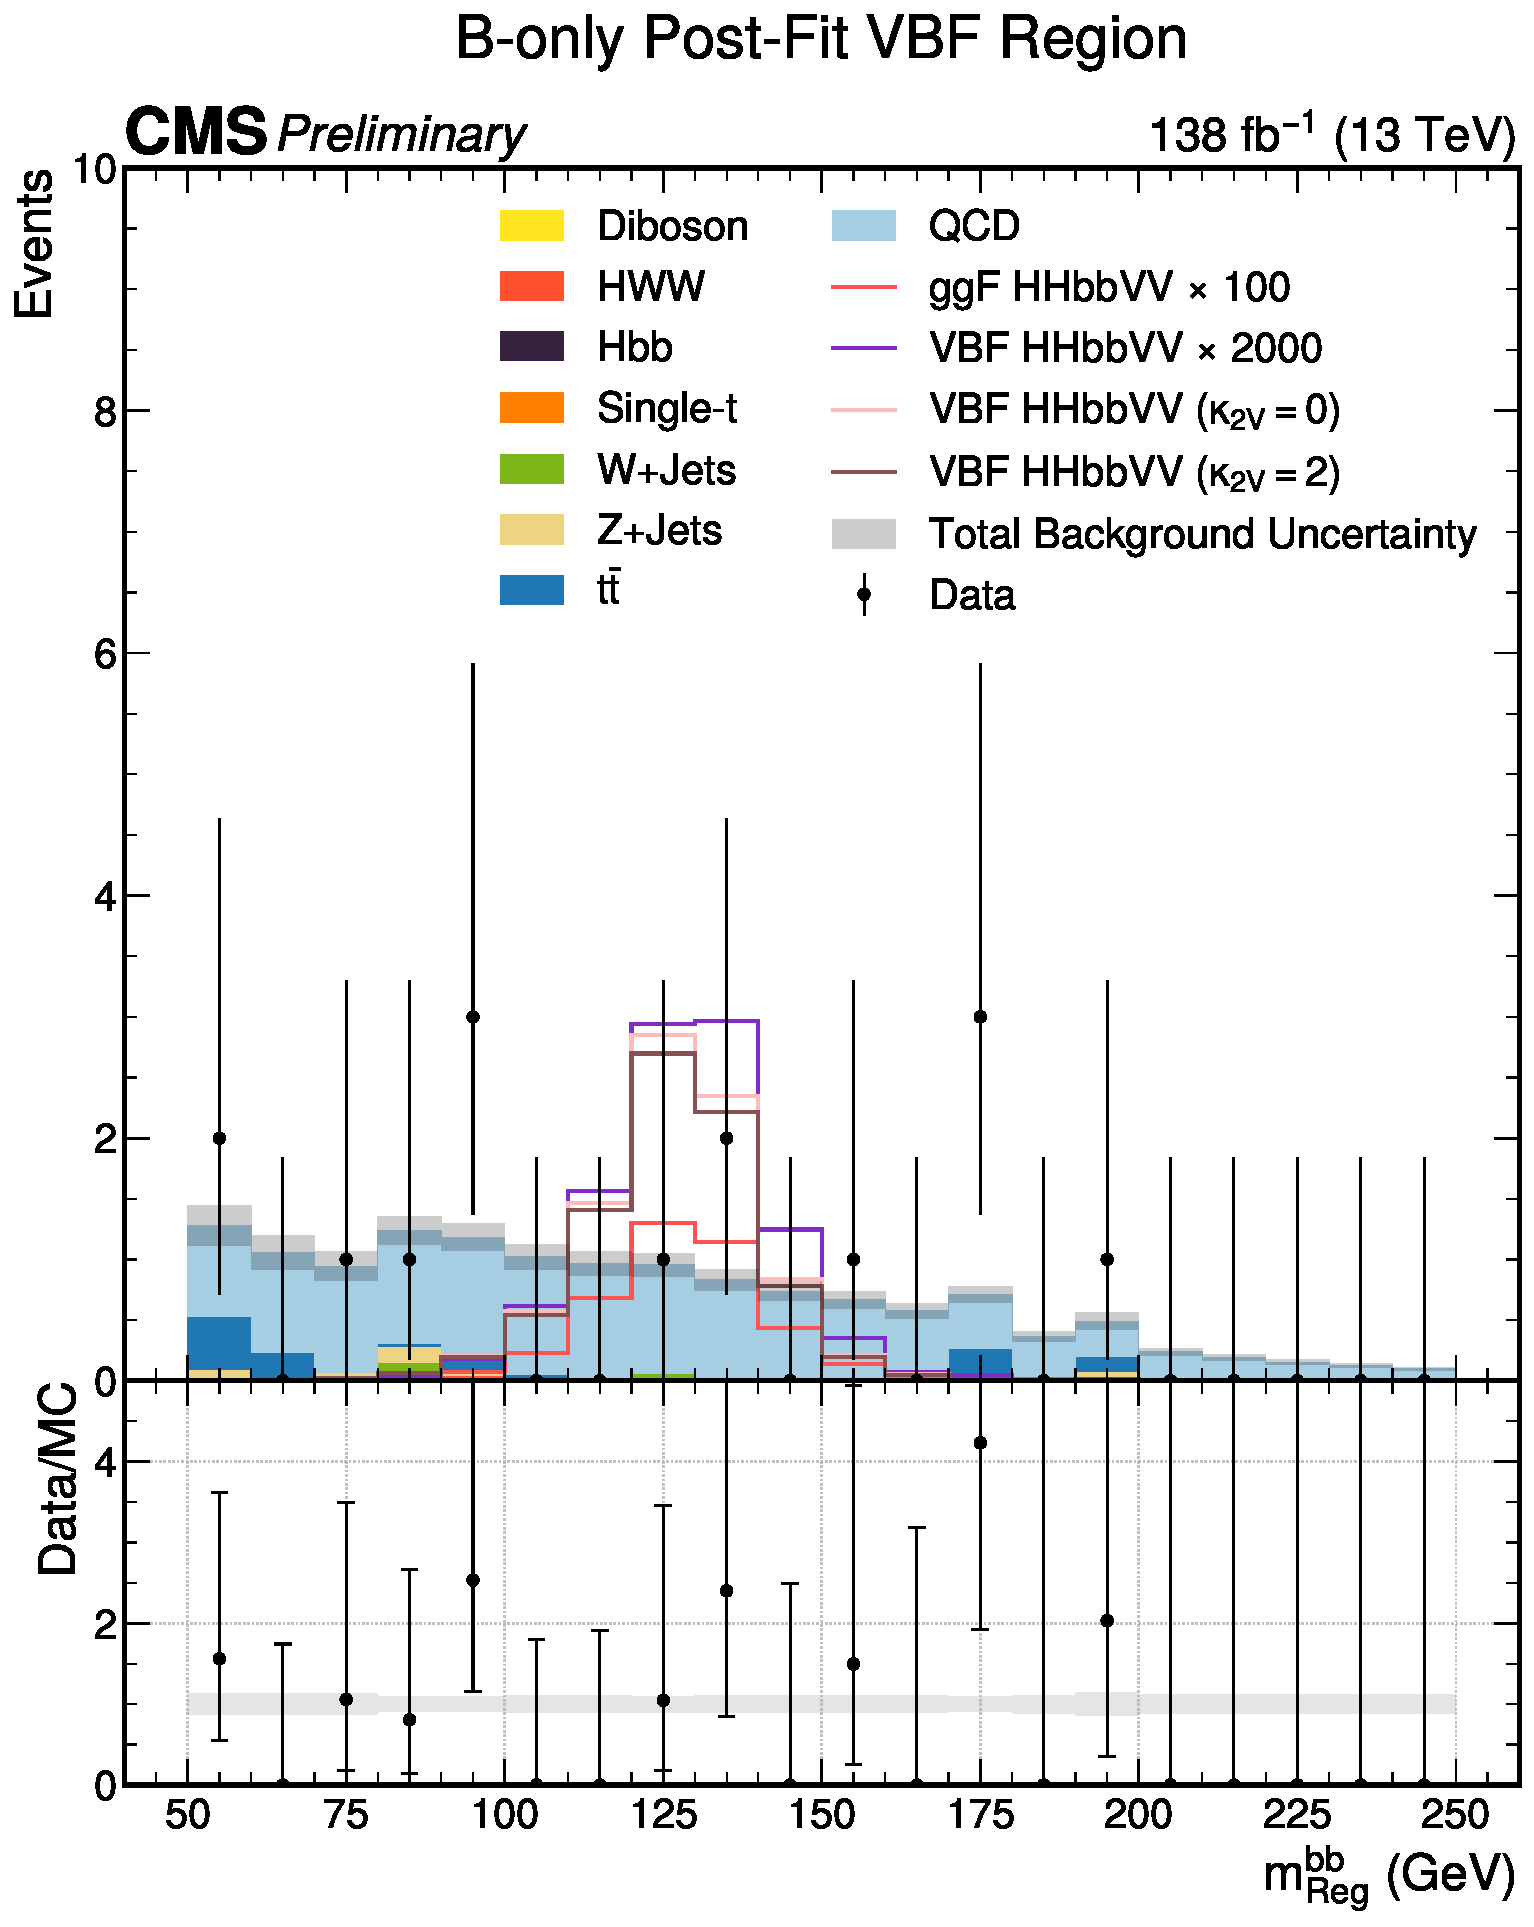
\includegraphics[trim={0 0 0 15mm},clip,width=0.49\textwidth]{figures/05-HH/results_nonres/postfit_passvbf_bbFatJetParticleNetMass.pdf}
\caption{Post-background-only-fit distributions of the \bbbar-candidate jet regressed mass (\mregbb) in the ggF (left) and VBF (right) signal regions.
The data is not shown in the Higgs mass window.
\label{fig:05_results_hh_postfit}
}
\end{figure}

\begin{figure}[hbt!]
\centering
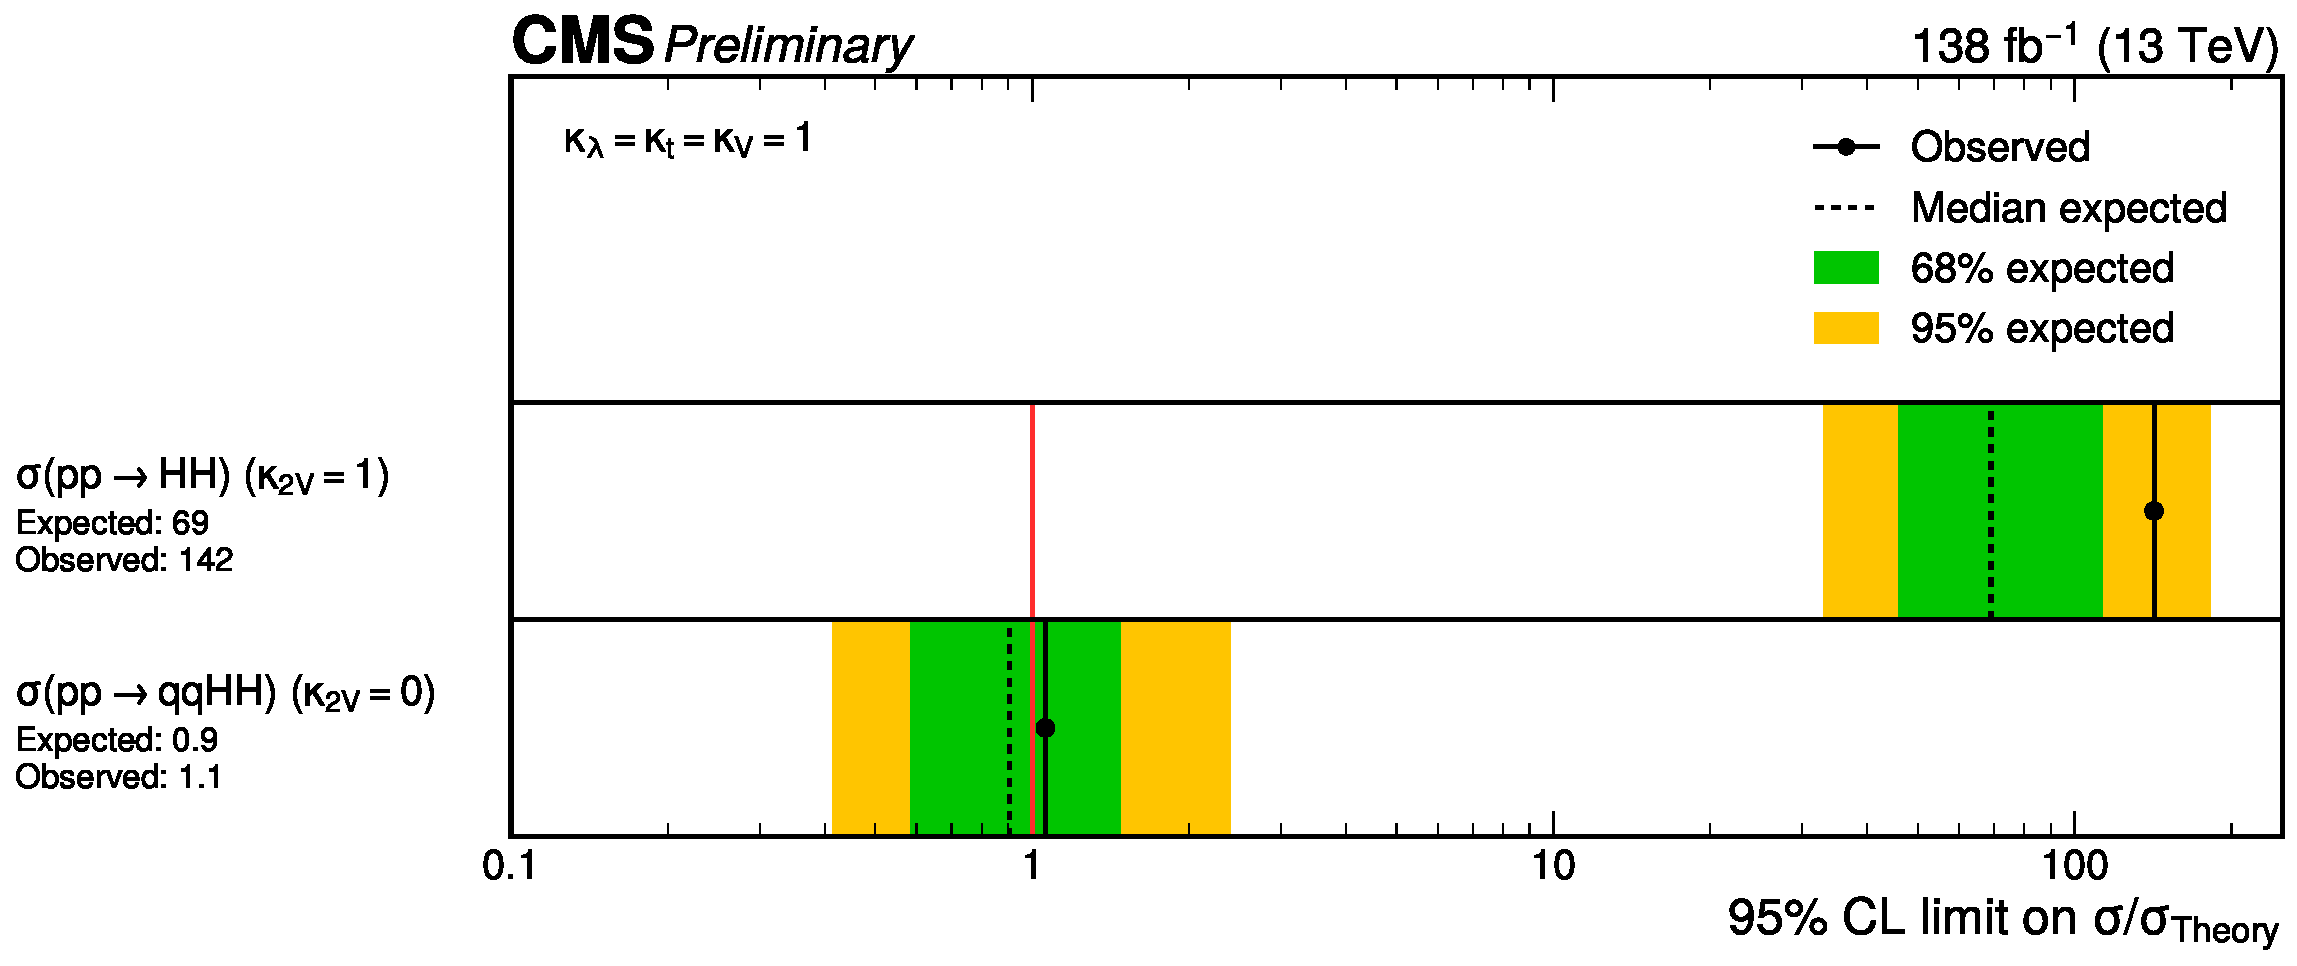
\includegraphics[width=\textwidth]{figures/05-HH/results_nonres/UL_combined.pdf}
\caption{Observed and expected exclusion limits at 95\% CL for the \HHbbVV signal SM cross section (top) and cross section at $\kapvv=0$ (bottom).
\label{fig:05_results_hh_UL}
}
\end{figure}

\begin{figure}[hbt!]
\centering
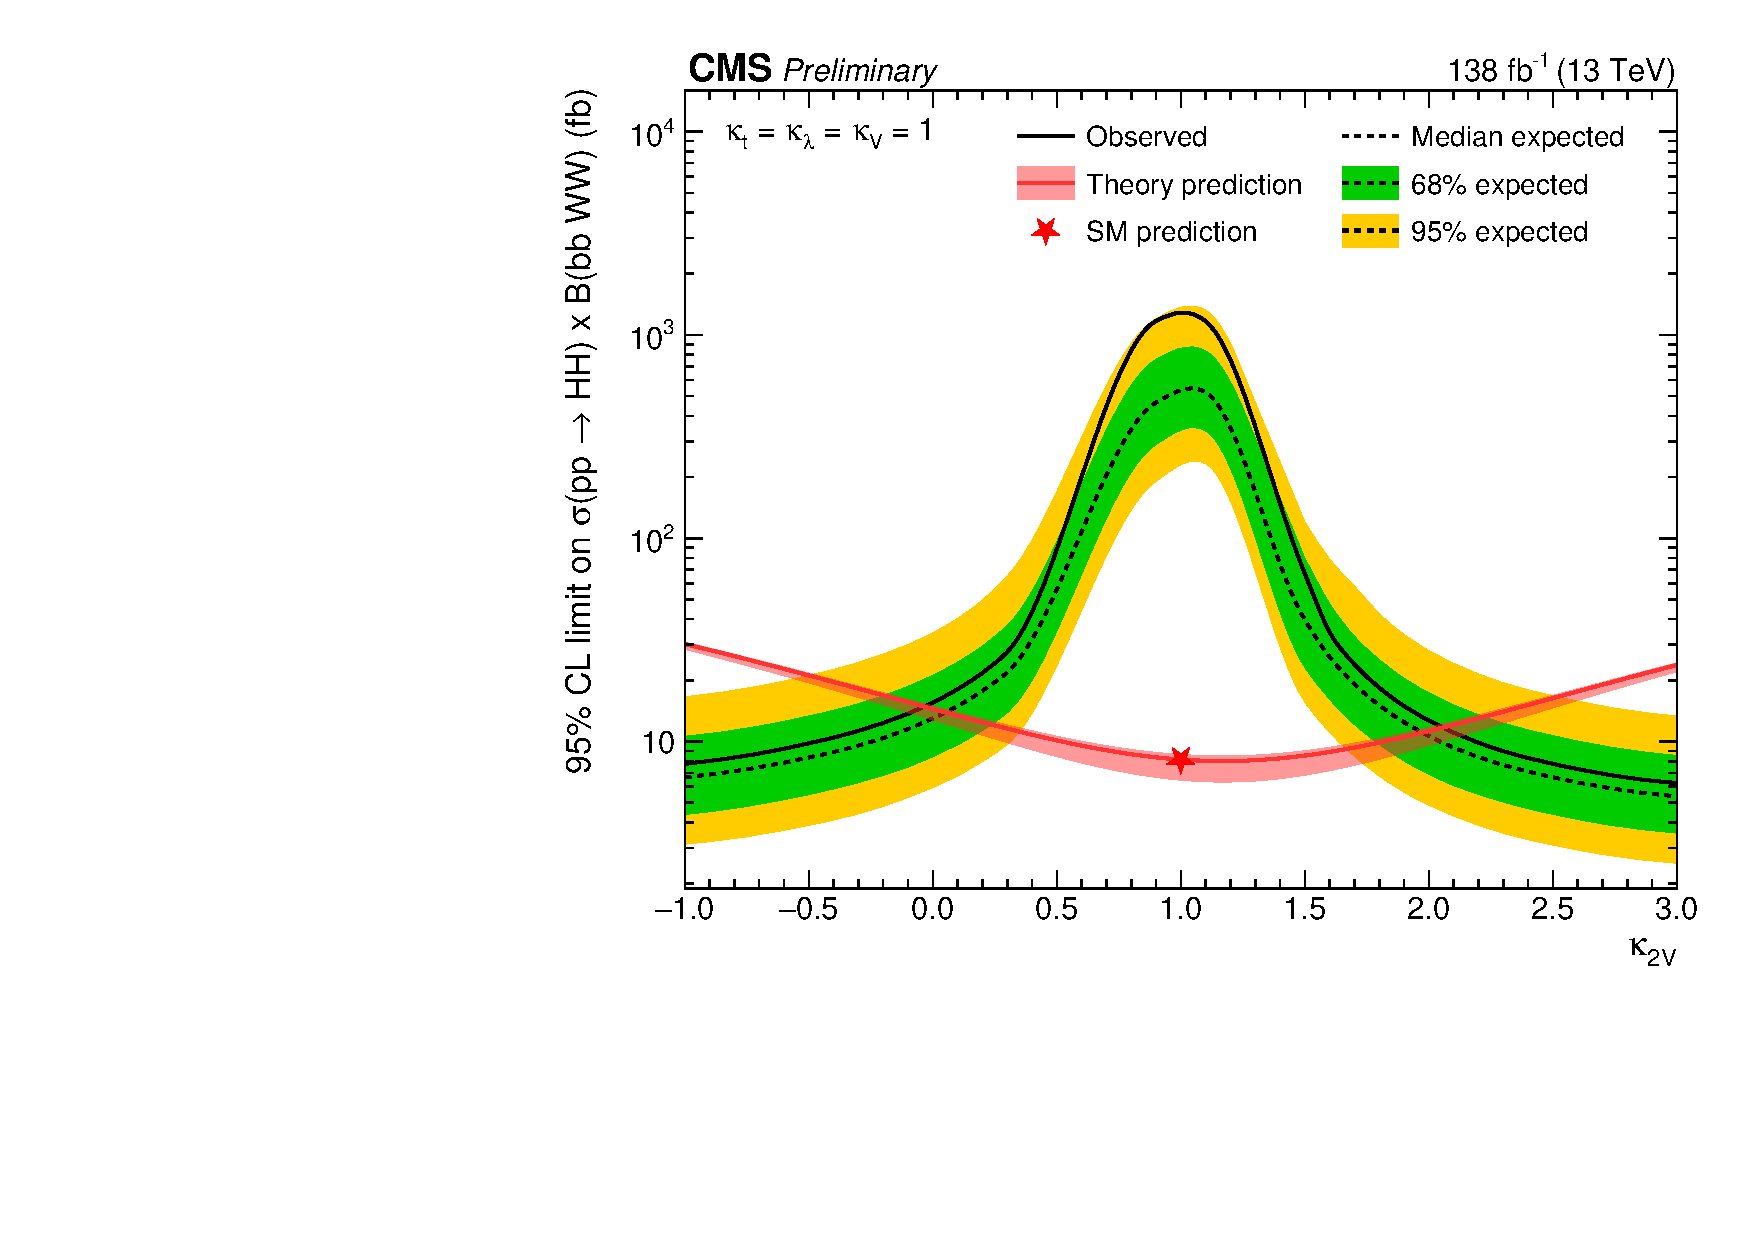
\includegraphics[width=0.7\textwidth]{figures/05-HH/results_nonres/UL_scan_C2V.pdf}
\caption{1D upper limits scans on the inclusive HH cross section as a function of \kapvv.
\label{fig:05_results_hh_UL_k2v}
}
\end{figure}


\subsection{Resonant \texorpdfstring{\XHY}{XHY} search}
\label{sec:05_results_xhy}

Similarly, a binned maximum likelihood fit is performed to the observed \mxmy distributions for a wide range of potential \PX and \PY mass points simultaneously in the fail and pass regions for the resonant analysis.
The data and post-fit estimates for the backgrounds are shown in Figure~\ref{fig:05_results_xhy_postfit_fm_mvv}, with the data not shown in the pass region as the analysis is currently blinded.
Upper limits on the \XHY production cross section, assuming a 100\% branching fraction for the \yvv decay, are shown in Figures~\ref{fig:05_results_xhy_xUL_fm}.


\begin{figure}[hbt!]
\centering
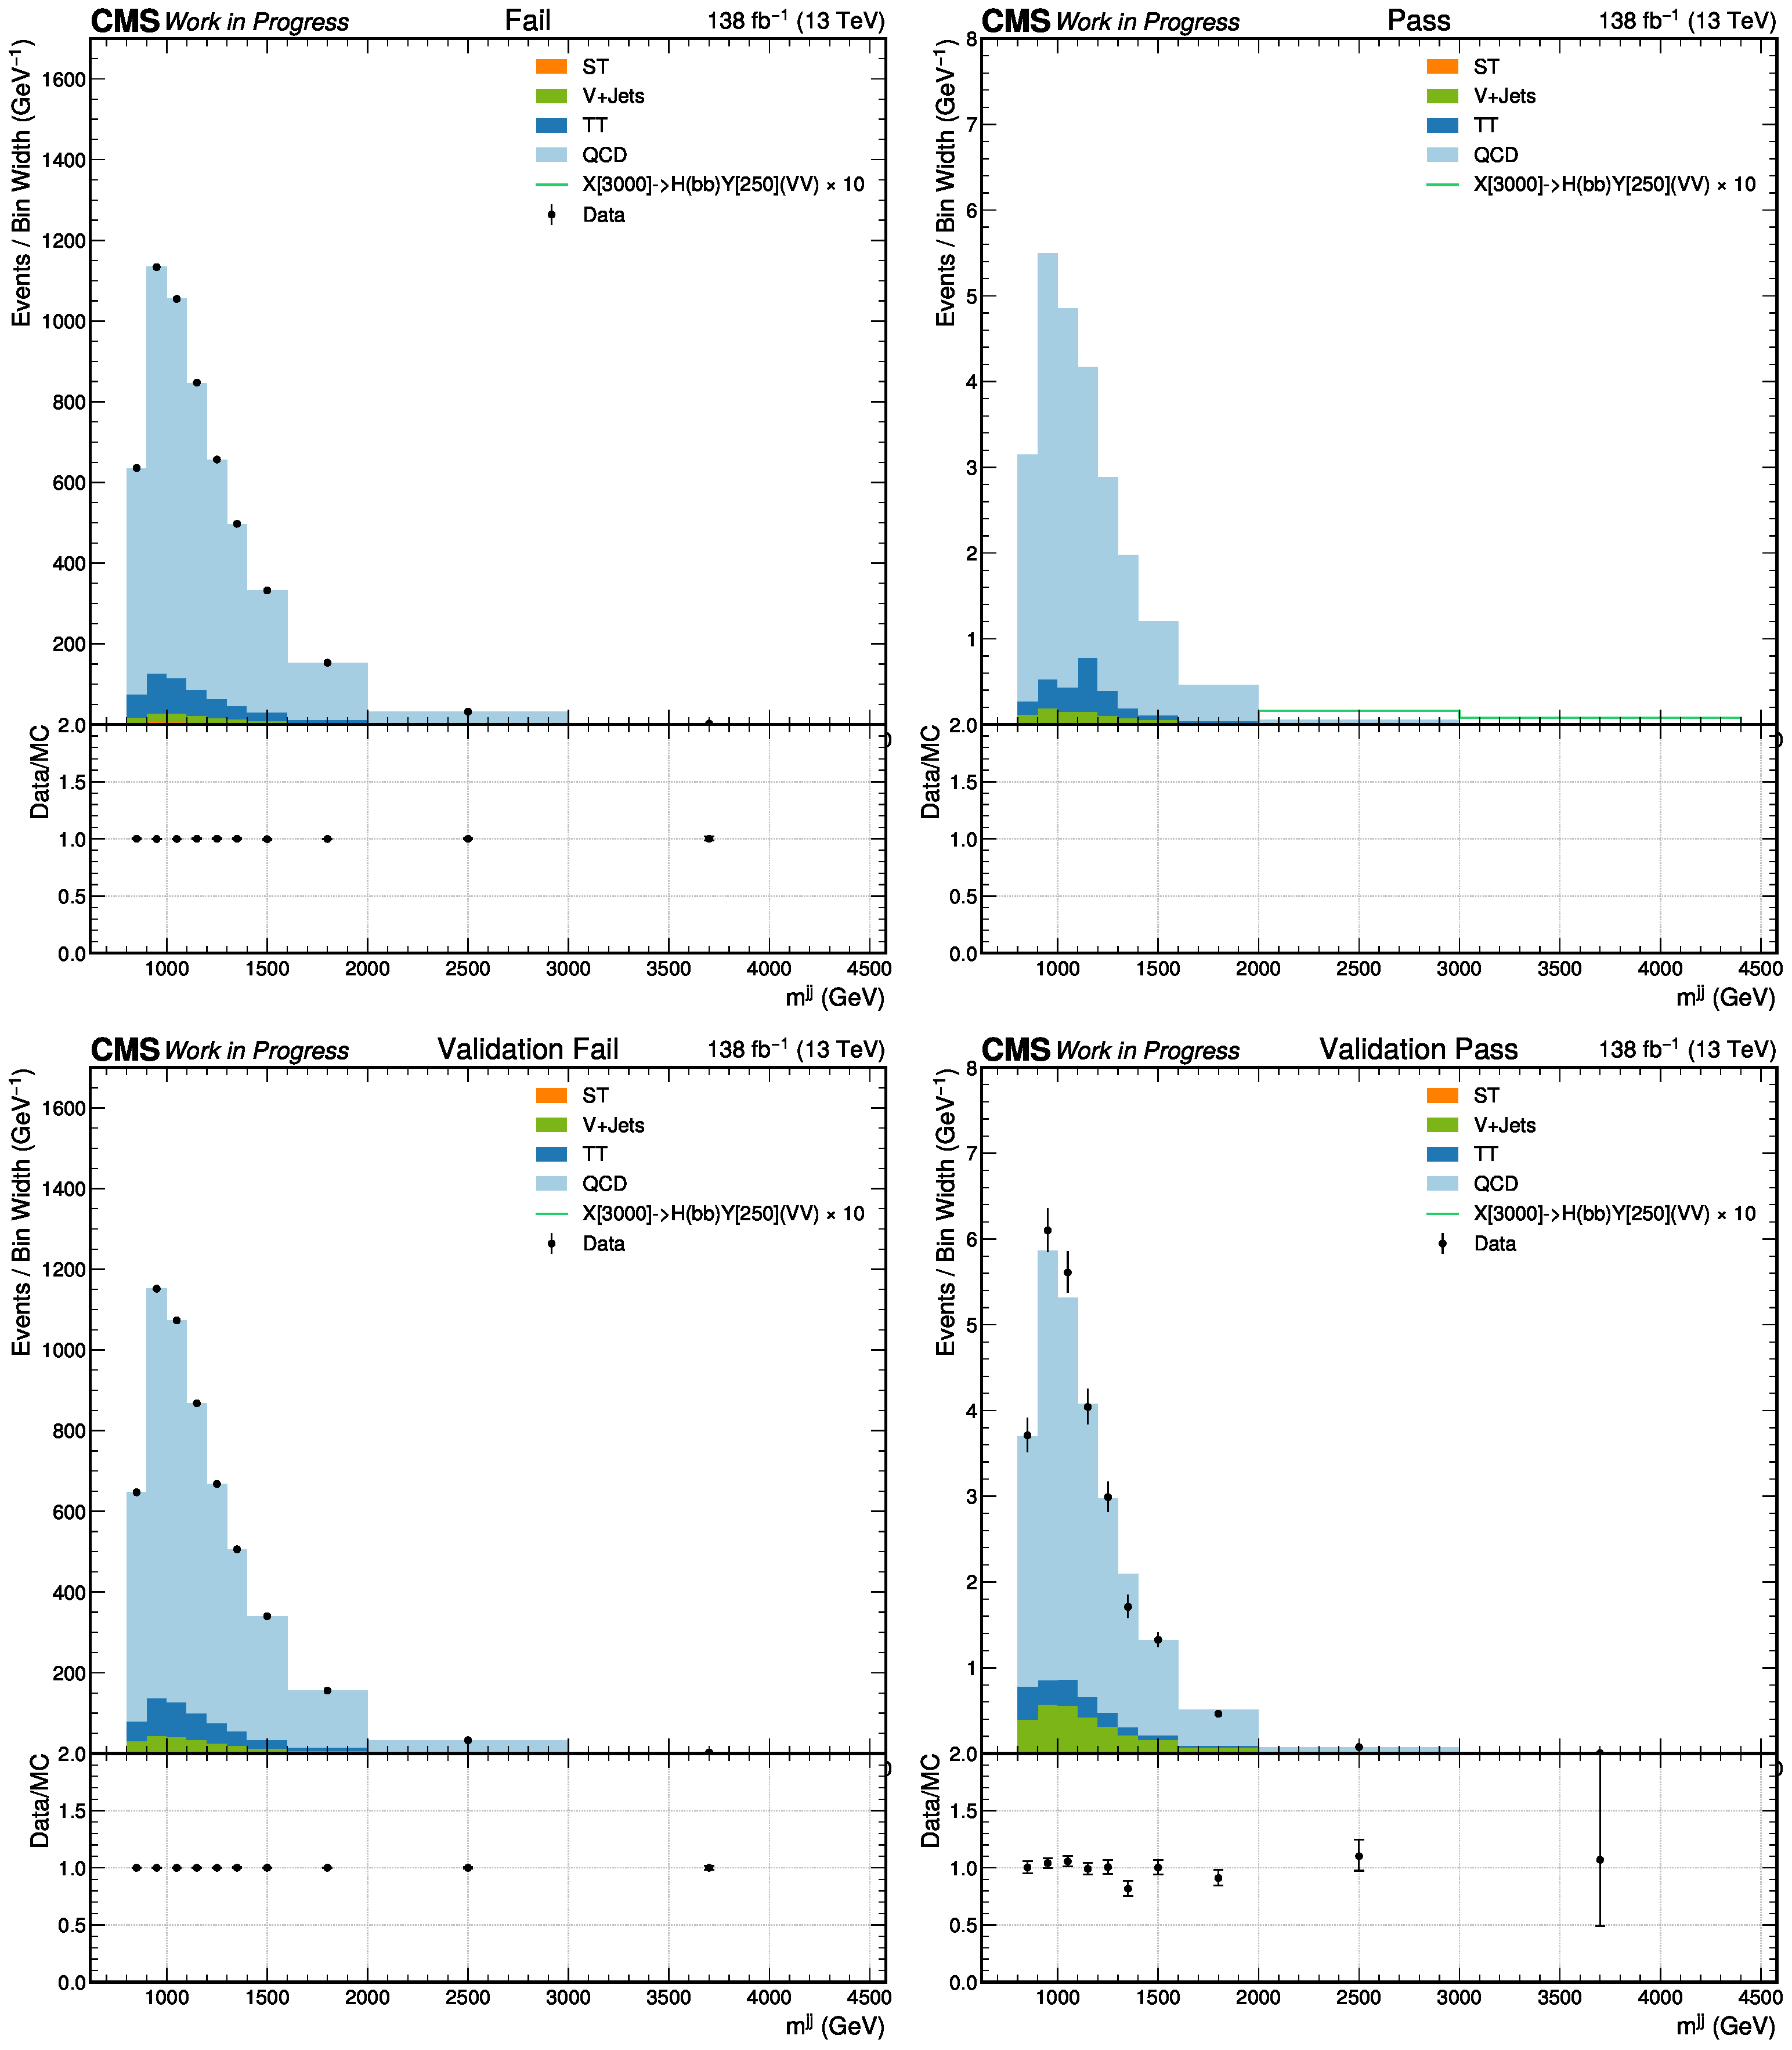
\includegraphics[width=\textwidth]{figures/05-HH/results_res/postfit_DijetMass.pdf}
\caption[Post-background-only-fit distributions in the fully-merged category of the \VV-candidate jet regressed mass (\mregvv).]{Post-background-only-fit distributions in the fully-merged category of the \VV-candidate jet regressed mass (\mregvv) in the validation fail (bottom left), and validation pass (bottom right) regions, as well as distributions in the pass region after applying the post-fit transfer factor from the validation regions (top right), and the fail region (top left).
The data is not shown in the pass region.
\label{fig:05_results_xhy_postfit_fm_mvv}
}
\end{figure}

\begin{figure}[hbt!]
\centering
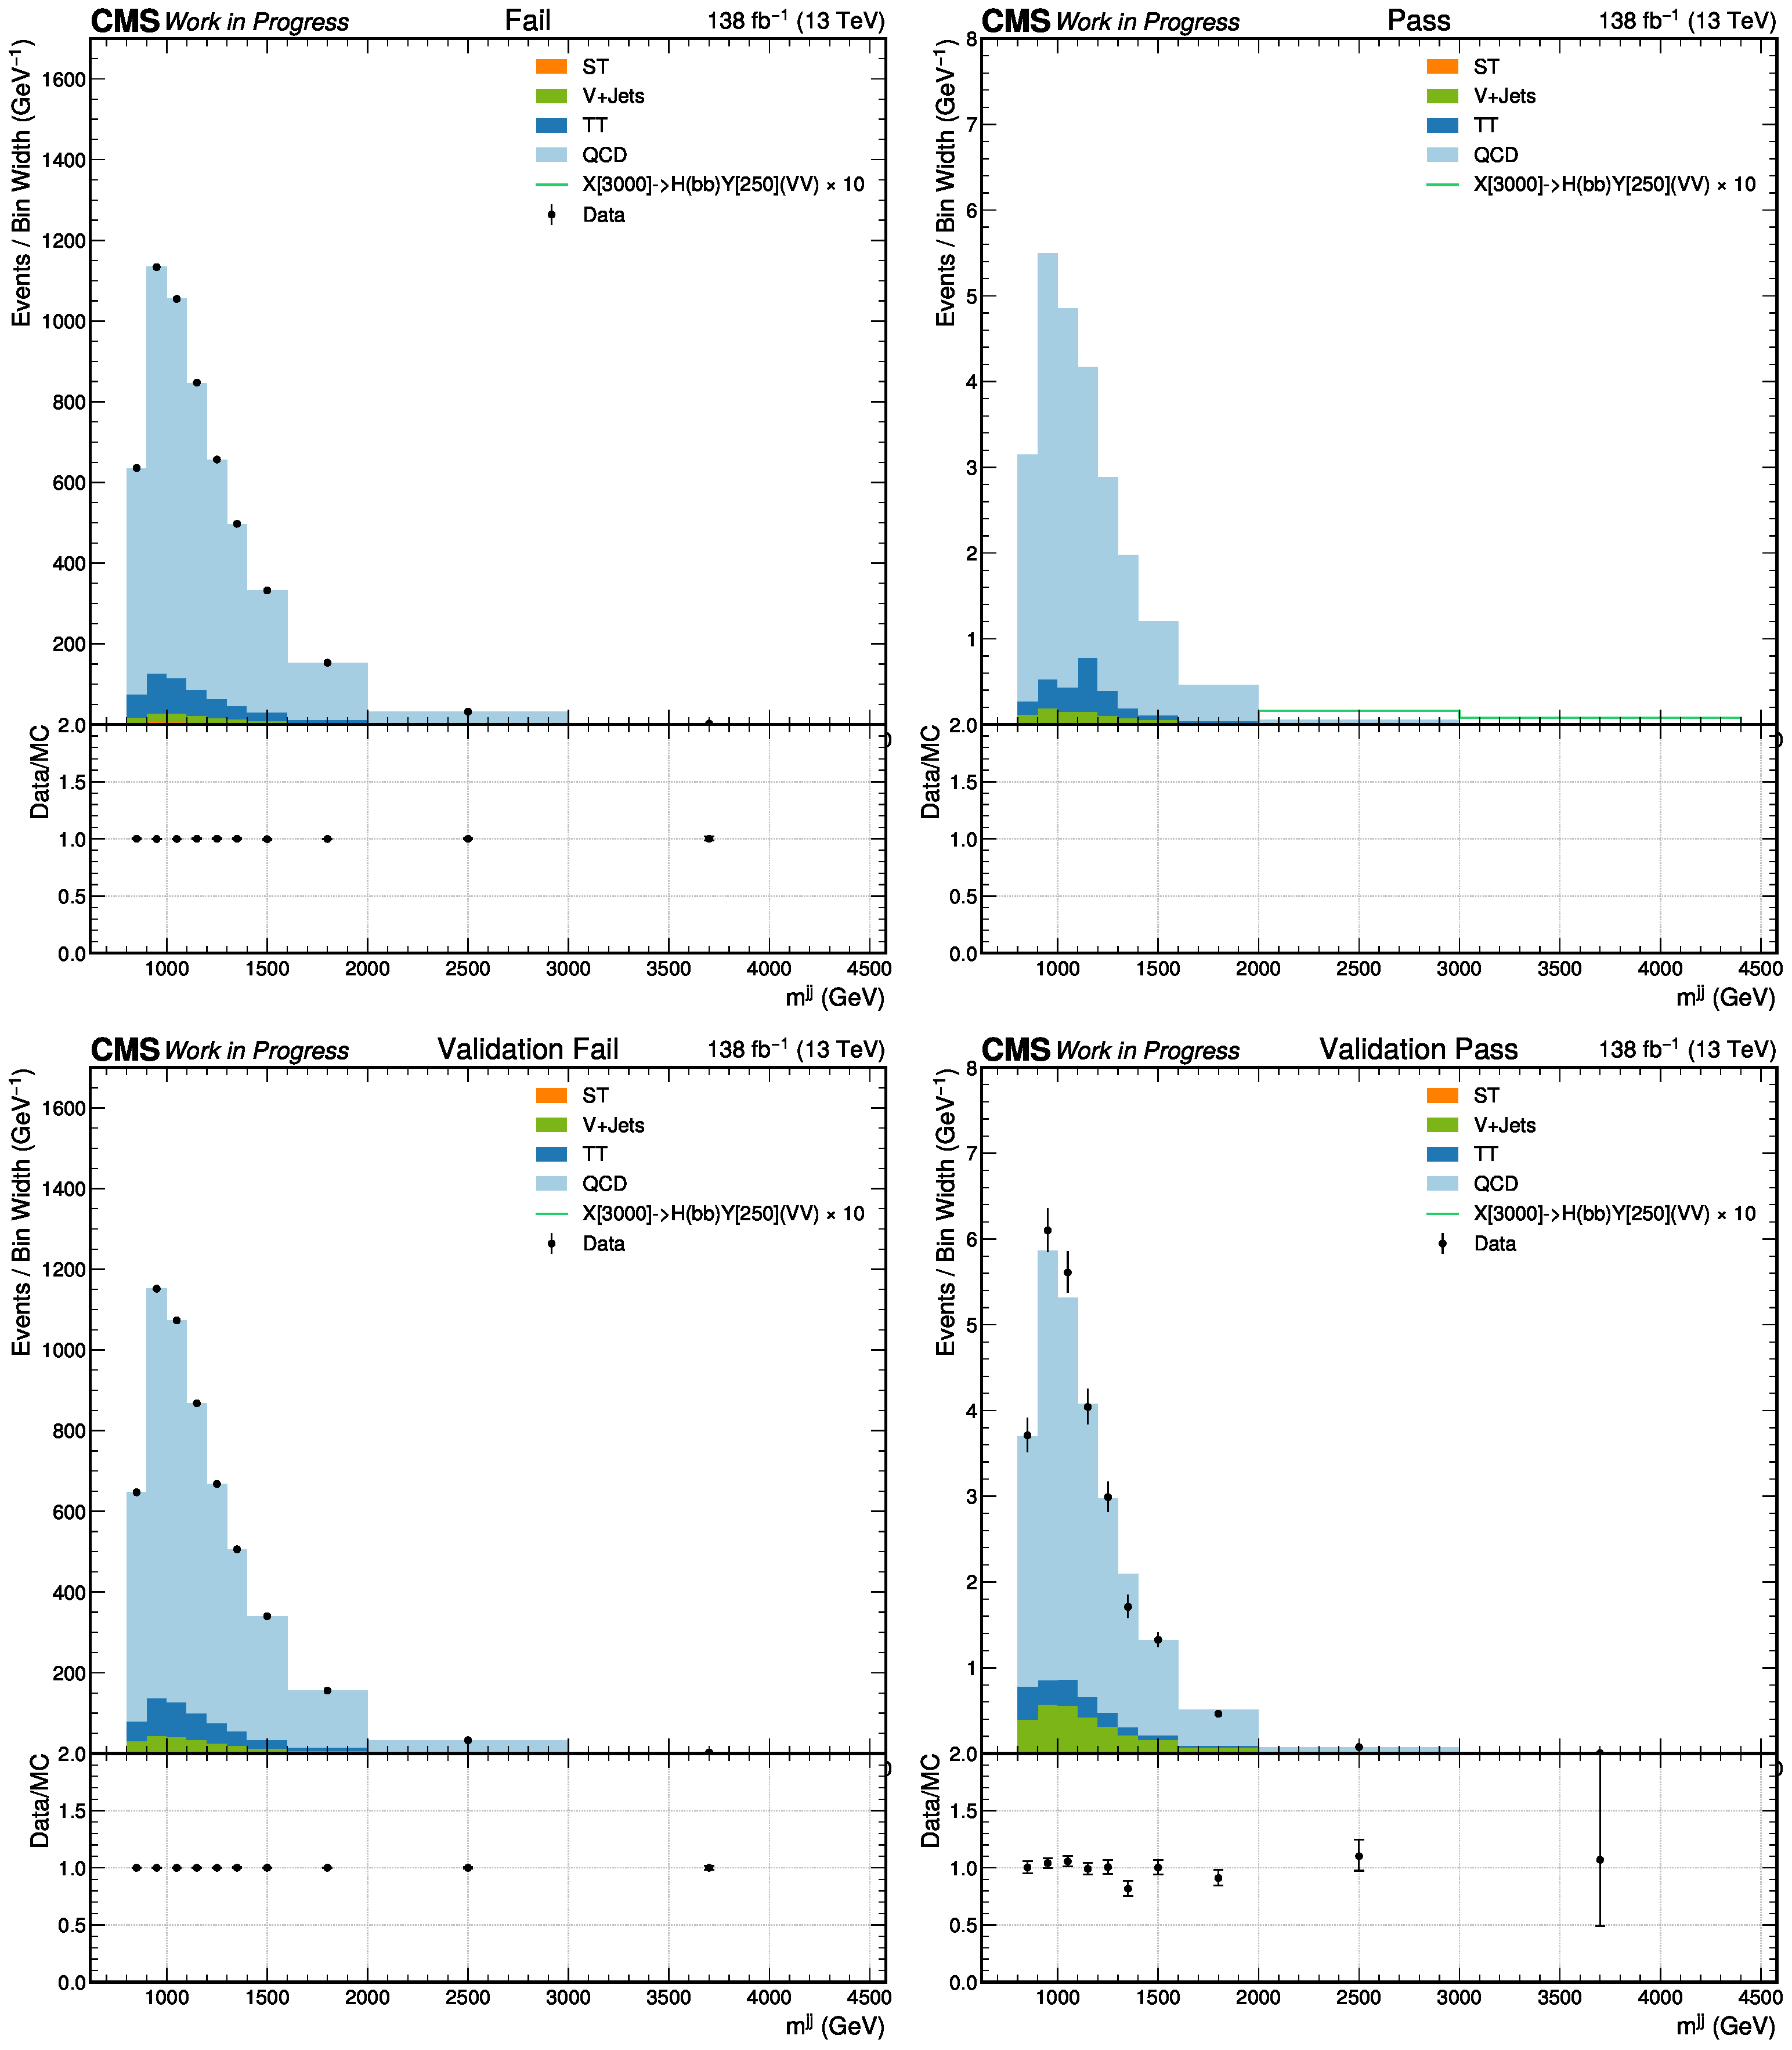
\includegraphics[width=\textwidth]{figures/05-HH/results_res/postfit_DijetMass.pdf}
\caption[Post-background-only-fit distributions in the fully-merged category of the dijet mass (\mjj).]{Post-background-only-fit distributions in the fully-merged category of the dijet mass (\mjj) in the validation fail (bottom left), and validation pass (bottom right) regions, as well as distributions in the pass region after applying the post-fit transfer factor from the validation regions (top right), and the fail region (top left).
The data is not shown in the pass region.
\label{fig:05_results_xhy_postfit_fm_mjj}
}
\end{figure}

\begin{figure}[hbt!]
\centering
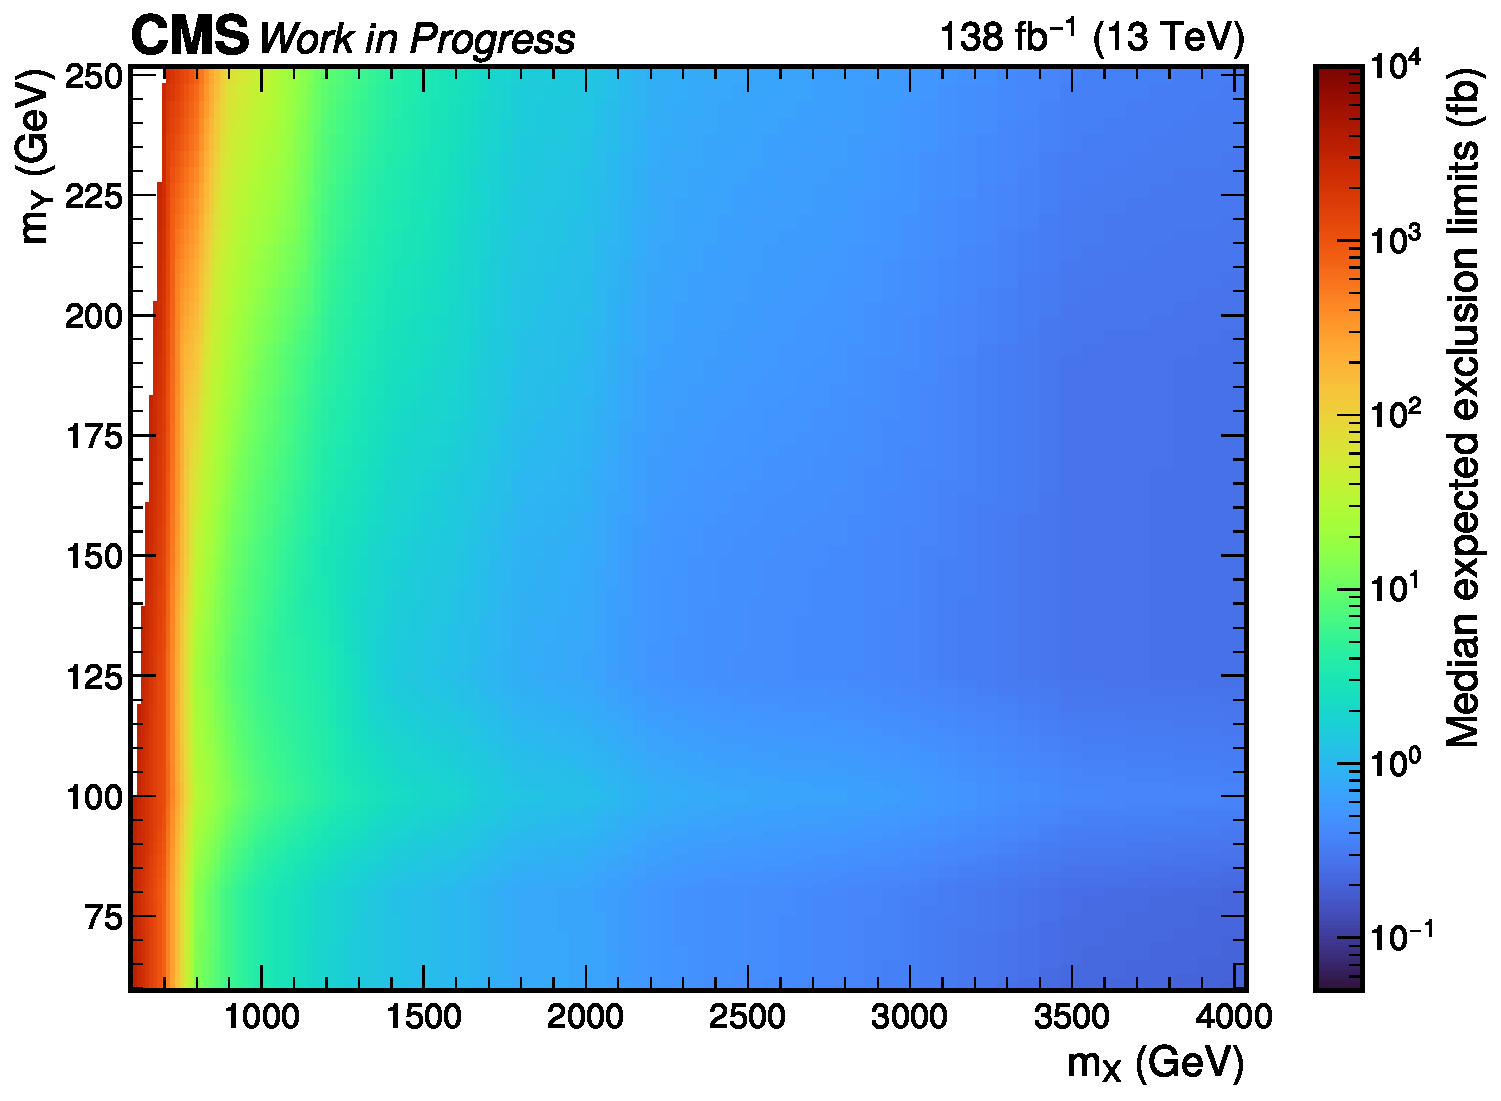
\includegraphics[width=\textwidth]{figures/05-HH/results_res/mesh_50.0_turbo.pdf}
\caption{Median expected exclusion limits in the fully-merged category for resonant \XHYbbVVq signals for different \mx and \my.
\label{fig:05_results_xhy_xUL_fm}
}
\end{figure}


% \section{Run 3 HH→4b}
% \label{sec:05_hh4b}

% As discussed in Section~\ref{sec:05_triggers}, a significant limitation of both the Run 2 boosted $\HH\to\bbvv$ and \bbbb analyses were the lack of dedicated triggers for boosted Higgs jets, leading to very low trigger efficiencies for AK8 jet $\pt < 400\GeV$.
% This has been improved in Run 3 with dedicated triggers boosted \hbb triggers using ParticleNet.
% The improvement in the trigger and the impact on the signal efficiency is shown in \TODO{Add if approved}.

\section{Summary and Outlook}
\label{sec:05_outlook}

In this chapter, we described two sensitive and complementary searches for SM nonresonant double Higgs boson production (\HH) and the BSM nonresonant massive scalar resonances \PX and \PY (\XHY), into the \bbbar and \VV all-hadronic final states, at high \mHH, and high \mx and \my, respectively.
The former aims to constrain the \kapvv quartic coupling modifier, while the latter is motivated by the high branching fraction predicted for the \yvv decay and the potential for new physics in the \XHY sector.

In both cases we search for boosted \HHY with fully merged jets; i.e., where all \PH and \PY daughter quarks are contained within a single wide-radius AK8 jet.
The established ParticleNet mass-decorrelated tagger is used to select for \hbb jets and we develop a new high performing Particle Transformer tagger for \hyvv jets.

We extract the SM \HH signal from the \hbb regressed mass and the resonant \XHY signal from the \yww regressed mass and dijet \PX mass, using control regions with tagger scores inverted to obtain a data-driven estimate of the shape and normalization of the QCD multijet background via a parametric transfer function.
Other minor backgrounds including top quark and vector boson plus jets are estimated using MC simulations.
We observe (expect) an upper limit at 95\% CL of $\hhobs\times$ ($\hhexp\times$) the SM for nonresonant \HHbbVVq production and a constraint on \kapvv of \kvvobslims (\kvvexplims), which is the second-highest constraint set by the CMS experiment.
We expect exclusion limits as low as 0.3fb for resonant \XHYbbVVq production for various \mx and \my mass points.

As discussed in Section~\ref{sec:05_triggers}, a significant limitation of both the Run 2 boosted $\HH\to\bbvv$ and \bbbb analyses were the lack of dedicated triggers for boosted Higgs jets, leading to very low trigger efficiencies for AK8 jet $\pt < 400\GeV$.
This has been improved in Run 3 with dedicated triggers boosted \hbb triggers using ParticleNet~\cite{Varghese:2023bue}, which have the potential to significantly improve our constraints on the \HH cross section and \kapvv.
Additionally, as the boosted regime is currently statistically limited, with the statistical uncertainty on the background estimate dominating the uncertainties on the signal strength, such boosted \HH analyses stand to gain significantly from the increased luminosity of Run 3 and HL-LHC as well.
Thus, the future is very bright for high energy searches of Higgs pair production!
% in the coming decade.
% \TODO{Discuss more if approved.}

\subsubsection{Acknowledgements}

This chapter, in part, is currently being prepared for the publication of the material by the CMS collaboration.
The dissertation author was the primary investigator and author of these papers.
